\PassOptionsToPackage{unicode=true}{hyperref} % options for packages loaded elsewhere
\PassOptionsToPackage{hyphens}{url}
%
\documentclass[ignorenonframetext,]{beamer}
\usepackage{pgfpages}
\setbeamertemplate{caption}[numbered]
\setbeamertemplate{caption label separator}{: }
\setbeamercolor{caption name}{fg=normal text.fg}
\beamertemplatenavigationsymbolsempty
% Prevent slide breaks in the middle of a paragraph:
\widowpenalties 1 10000
\raggedbottom
\setbeamertemplate{part page}{
\centering
\begin{beamercolorbox}[sep=16pt,center]{part title}
  \usebeamerfont{part title}\insertpart\par
\end{beamercolorbox}
}
\setbeamertemplate{section page}{
\centering
\begin{beamercolorbox}[sep=12pt,center]{part title}
  \usebeamerfont{section title}\insertsection\par
\end{beamercolorbox}
}
\setbeamertemplate{subsection page}{
\centering
\begin{beamercolorbox}[sep=8pt,center]{part title}
  \usebeamerfont{subsection title}\insertsubsection\par
\end{beamercolorbox}
}
\AtBeginPart{
  \frame{\partpage}
}
\AtBeginSection{
  \ifbibliography
  \else
    \frame{\sectionpage}
  \fi
}
\AtBeginSubsection{
  \frame{\subsectionpage}
}
\usepackage{lmodern}
\usepackage{amssymb,amsmath}
\usepackage{ifxetex,ifluatex}
\usepackage{fixltx2e} % provides \textsubscript
\ifnum 0\ifxetex 1\fi\ifluatex 1\fi=0 % if pdftex
  \usepackage[T1]{fontenc}
  \usepackage[utf8]{inputenc}
  \usepackage{textcomp} % provides euro and other symbols
\else % if luatex or xelatex
  \usepackage{unicode-math}
  \defaultfontfeatures{Ligatures=TeX,Scale=MatchLowercase}
\fi
\usetheme[]{AnnArbor}
\usecolortheme{dove}
% use upquote if available, for straight quotes in verbatim environments
\IfFileExists{upquote.sty}{\usepackage{upquote}}{}
% use microtype if available
\IfFileExists{microtype.sty}{%
\usepackage[]{microtype}
\UseMicrotypeSet[protrusion]{basicmath} % disable protrusion for tt fonts
}{}
\IfFileExists{parskip.sty}{%
\usepackage{parskip}
}{% else
\setlength{\parindent}{0pt}
\setlength{\parskip}{6pt plus 2pt minus 1pt}
}
\usepackage{hyperref}
\hypersetup{
            pdftitle={STAD29: Statistics for the Life and Social Sciences},
            pdfauthor={Lecture notes},
            pdfborder={0 0 0},
            breaklinks=true}
\urlstyle{same}  % don't use monospace font for urls
\newif\ifbibliography
\usepackage{color}
\usepackage{fancyvrb}
\newcommand{\VerbBar}{|}
\newcommand{\VERB}{\Verb[commandchars=\\\{\}]}
\DefineVerbatimEnvironment{Highlighting}{Verbatim}{commandchars=\\\{\}}
% Add ',fontsize=\small' for more characters per line
\usepackage{framed}
\definecolor{shadecolor}{RGB}{248,248,248}
\newenvironment{Shaded}{\begin{snugshade}}{\end{snugshade}}
\newcommand{\AlertTok}[1]{\textcolor[rgb]{0.94,0.16,0.16}{#1}}
\newcommand{\AnnotationTok}[1]{\textcolor[rgb]{0.56,0.35,0.01}{\textbf{\textit{#1}}}}
\newcommand{\AttributeTok}[1]{\textcolor[rgb]{0.77,0.63,0.00}{#1}}
\newcommand{\BaseNTok}[1]{\textcolor[rgb]{0.00,0.00,0.81}{#1}}
\newcommand{\BuiltInTok}[1]{#1}
\newcommand{\CharTok}[1]{\textcolor[rgb]{0.31,0.60,0.02}{#1}}
\newcommand{\CommentTok}[1]{\textcolor[rgb]{0.56,0.35,0.01}{\textit{#1}}}
\newcommand{\CommentVarTok}[1]{\textcolor[rgb]{0.56,0.35,0.01}{\textbf{\textit{#1}}}}
\newcommand{\ConstantTok}[1]{\textcolor[rgb]{0.00,0.00,0.00}{#1}}
\newcommand{\ControlFlowTok}[1]{\textcolor[rgb]{0.13,0.29,0.53}{\textbf{#1}}}
\newcommand{\DataTypeTok}[1]{\textcolor[rgb]{0.13,0.29,0.53}{#1}}
\newcommand{\DecValTok}[1]{\textcolor[rgb]{0.00,0.00,0.81}{#1}}
\newcommand{\DocumentationTok}[1]{\textcolor[rgb]{0.56,0.35,0.01}{\textbf{\textit{#1}}}}
\newcommand{\ErrorTok}[1]{\textcolor[rgb]{0.64,0.00,0.00}{\textbf{#1}}}
\newcommand{\ExtensionTok}[1]{#1}
\newcommand{\FloatTok}[1]{\textcolor[rgb]{0.00,0.00,0.81}{#1}}
\newcommand{\FunctionTok}[1]{\textcolor[rgb]{0.00,0.00,0.00}{#1}}
\newcommand{\ImportTok}[1]{#1}
\newcommand{\InformationTok}[1]{\textcolor[rgb]{0.56,0.35,0.01}{\textbf{\textit{#1}}}}
\newcommand{\KeywordTok}[1]{\textcolor[rgb]{0.13,0.29,0.53}{\textbf{#1}}}
\newcommand{\NormalTok}[1]{#1}
\newcommand{\OperatorTok}[1]{\textcolor[rgb]{0.81,0.36,0.00}{\textbf{#1}}}
\newcommand{\OtherTok}[1]{\textcolor[rgb]{0.56,0.35,0.01}{#1}}
\newcommand{\PreprocessorTok}[1]{\textcolor[rgb]{0.56,0.35,0.01}{\textit{#1}}}
\newcommand{\RegionMarkerTok}[1]{#1}
\newcommand{\SpecialCharTok}[1]{\textcolor[rgb]{0.00,0.00,0.00}{#1}}
\newcommand{\SpecialStringTok}[1]{\textcolor[rgb]{0.31,0.60,0.02}{#1}}
\newcommand{\StringTok}[1]{\textcolor[rgb]{0.31,0.60,0.02}{#1}}
\newcommand{\VariableTok}[1]{\textcolor[rgb]{0.00,0.00,0.00}{#1}}
\newcommand{\VerbatimStringTok}[1]{\textcolor[rgb]{0.31,0.60,0.02}{#1}}
\newcommand{\WarningTok}[1]{\textcolor[rgb]{0.56,0.35,0.01}{\textbf{\textit{#1}}}}
\usepackage{graphicx,grffile}
\makeatletter
\def\maxwidth{\ifdim\Gin@nat@width>\linewidth\linewidth\else\Gin@nat@width\fi}
\def\maxheight{\ifdim\Gin@nat@height>\textheight\textheight\else\Gin@nat@height\fi}
\makeatother
% Scale images if necessary, so that they will not overflow the page
% margins by default, and it is still possible to overwrite the defaults
% using explicit options in \includegraphics[width, height, ...]{}
\setkeys{Gin}{width=\maxwidth,height=\maxheight,keepaspectratio}
\setlength{\emergencystretch}{3em}  % prevent overfull lines
\providecommand{\tightlist}{%
  \setlength{\itemsep}{0pt}\setlength{\parskip}{0pt}}
\setcounter{secnumdepth}{0}

% set default figure placement to htbp
\makeatletter
\def\fps@figure{htbp}
\makeatother

\usepackage{multicol}

\title{STAD29: Statistics for the Life and Social Sciences}
\author{Lecture notes}
\date{}

\begin{document}
\frame{\titlepage}

\hypertarget{principal-components}{%
\section{Principal components}\label{principal-components}}

\begin{frame}{Principal Components}
\protect\hypertarget{principal-components-1}{}

\begin{itemize}
\item
  Have measurements on (possibly large) number of variables on some
  individuals.
\item
  Question: can we describe data using fewer variables (because original
  variables correlated in some way)?
\item
  Look for direction (linear combination of original variables) in which
  values \emph{most spread out}. This is \emph{first principal
  component}.
\item
  Second principal component then direction uncorrelated with this in
  which values then most spread out. And so on.
\end{itemize}

\end{frame}

\begin{frame}{Principal components}
\protect\hypertarget{principal-components-2}{}

\begin{itemize}
\item
  See whether small number of principal components captures most of
  variation in data.
\item
  Might try to interpret principal components.
\item
  If 2 components good, can make plot of data.
\item
  (Like discriminant analysis, but no groups.)
\item
  ``What are important ways that these data vary?''
\end{itemize}

\end{frame}

\begin{frame}[fragile]{Packages}
\protect\hypertarget{packages}{}

You might not have installed the first of these. See over for
instructions.

\begin{Shaded}
\begin{Highlighting}[]
\KeywordTok{library}\NormalTok{(ggbiplot) }\CommentTok{# see over}
\KeywordTok{library}\NormalTok{(tidyverse)}
\KeywordTok{library}\NormalTok{(ggrepel)}
\end{Highlighting}
\end{Shaded}

\end{frame}

\begin{frame}[fragile]{Installing \texttt{ggbiplot}}
\protect\hypertarget{installing-ggbiplot}{}

\begin{itemize}
\item
  \texttt{ggbiplot} not on CRAN, so usual \texttt{install.packages} will
  not work. This is same procedure you used for \texttt{smmr} in C32:
\item
  Install package \texttt{devtools} first (once):
\end{itemize}

\begin{Shaded}
\begin{Highlighting}[]
\KeywordTok{install.packages}\NormalTok{(}\StringTok{"devtools"}\NormalTok{)}
\end{Highlighting}
\end{Shaded}

\begin{itemize}
\tightlist
\item
  Then install \texttt{ggbiplot} (once):
\end{itemize}

\begin{Shaded}
\begin{Highlighting}[]
\KeywordTok{library}\NormalTok{(devtools)}
\KeywordTok{install_github}\NormalTok{(}\StringTok{"vqv/ggbiplot"}\NormalTok{)}
\end{Highlighting}
\end{Shaded}

\end{frame}

\begin{frame}[fragile]{Small example: 2 test scores for 8 people}
\protect\hypertarget{small-example-2-test-scores-for-8-people}{}

\small

\begin{Shaded}
\begin{Highlighting}[]
\NormalTok{my_url <-}\StringTok{ "http://www.utsc.utoronto.ca/~butler/d29/test12.txt"}
\NormalTok{test12 <-}\StringTok{ }\KeywordTok{read_table2}\NormalTok{(my_url)}
\NormalTok{test12}
\end{Highlighting}
\end{Shaded}

\begin{verbatim}
## # A tibble: 8 x 3
##   first second id   
##   <dbl>  <dbl> <chr>
## 1     2      9 A    
## 2    16     40 B    
## 3     8     17 C    
## 4    18     43 D    
## 5    10     25 E    
## 6     4     10 F    
## 7    10     27 G    
## 8    12     30 H
\end{verbatim}

\begin{Shaded}
\begin{Highlighting}[]
\NormalTok{g <-}\StringTok{ }\KeywordTok{ggplot}\NormalTok{(test12, }\KeywordTok{aes}\NormalTok{(}\DataTypeTok{x =}\NormalTok{ first, }\DataTypeTok{y =}\NormalTok{ second, }\DataTypeTok{label =}\NormalTok{ id)) }\OperatorTok{+}
\StringTok{  }\KeywordTok{geom_point}\NormalTok{() }\OperatorTok{+}\StringTok{ }\KeywordTok{geom_text_repel}\NormalTok{()}
\end{Highlighting}
\end{Shaded}

\normalsize

\end{frame}

\begin{frame}[fragile]{The plot}
\protect\hypertarget{the-plot}{}

\begin{Shaded}
\begin{Highlighting}[]
\NormalTok{g }\OperatorTok{+}\StringTok{ }\KeywordTok{geom_smooth}\NormalTok{(}\DataTypeTok{method =} \StringTok{"lm"}\NormalTok{, }\DataTypeTok{se =}\NormalTok{ F)}
\end{Highlighting}
\end{Shaded}

\begin{figure}
\centering
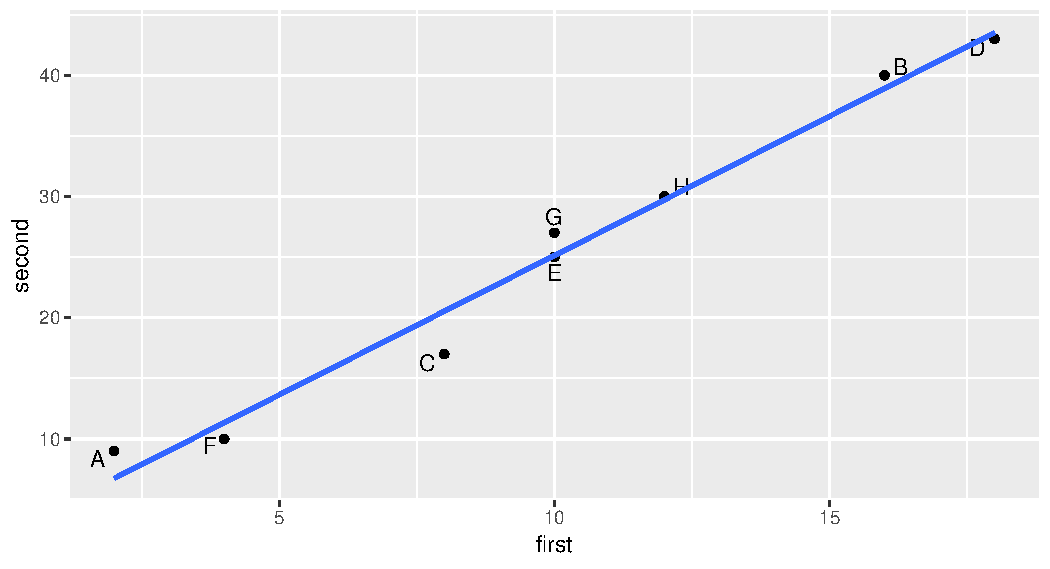
\includegraphics{figure/ff2-1.pdf}
\caption{plot of chunk ff2}
\end{figure}

\end{frame}

\begin{frame}[fragile]{Principal component analysis}
\protect\hypertarget{principal-component-analysis}{}

\begin{itemize}
\tightlist
\item
  Grab just the numeric columns:
\end{itemize}

\begin{Shaded}
\begin{Highlighting}[]
\NormalTok{test12 }\OperatorTok\StringTok{ }\KeywordTok{select_if}\NormalTok{(is.numeric) ->}\StringTok{ }\NormalTok{test12_numbers}
\end{Highlighting}
\end{Shaded}

\begin{itemize}
\tightlist
\item
  Strongly correlated, so data nearly 1-dimensional:
\end{itemize}

\begin{Shaded}
\begin{Highlighting}[]
\KeywordTok{cor}\NormalTok{(test12_numbers)}
\end{Highlighting}
\end{Shaded}

\begin{verbatim}
##           first   second
## first  1.000000 0.989078
## second 0.989078 1.000000
\end{verbatim}

\end{frame}

\begin{frame}[fragile]{Finding principal components}
\protect\hypertarget{finding-principal-components}{}

\begin{itemize}
\tightlist
\item
  Make a score summarizing this one dimension. Like this:
\end{itemize}

\begin{Shaded}
\begin{Highlighting}[]
\NormalTok{test12.pc <-}\StringTok{ }\KeywordTok{princomp}\NormalTok{(test12_numbers, }\DataTypeTok{cor =}\NormalTok{ T)}
\KeywordTok{summary}\NormalTok{(test12.pc)}
\end{Highlighting}
\end{Shaded}

\begin{verbatim}
## Importance of components:
##                          Comp.1      Comp.2
## Standard deviation     1.410347 0.104508582
## Proportion of Variance 0.994539 0.005461022
## Cumulative Proportion  0.994539 1.000000000
\end{verbatim}

\end{frame}

\begin{frame}[fragile]{Comments}
\protect\hypertarget{comments}{}

\begin{itemize}
\item
  ``Standard deviation'' shows relative importance of components (as for
  LDs in discriminant analysis)
\item
  Here, first one explains almost all (99.4\%) of variability.
\item
  That is, look only at first component and ignore second.
\item
  \texttt{cor=T} standardizes all variables first. Usually wanted,
  because variables measured on different scales. (Only omit if
  variables measured on same scale and expect similar variability.)
\end{itemize}

\end{frame}

\begin{frame}[fragile]{Scree plot}
\protect\hypertarget{scree-plot}{}

\begin{Shaded}
\begin{Highlighting}[]
\KeywordTok{ggscreeplot}\NormalTok{(test12.pc)}
\end{Highlighting}
\end{Shaded}

\begin{figure}
\centering
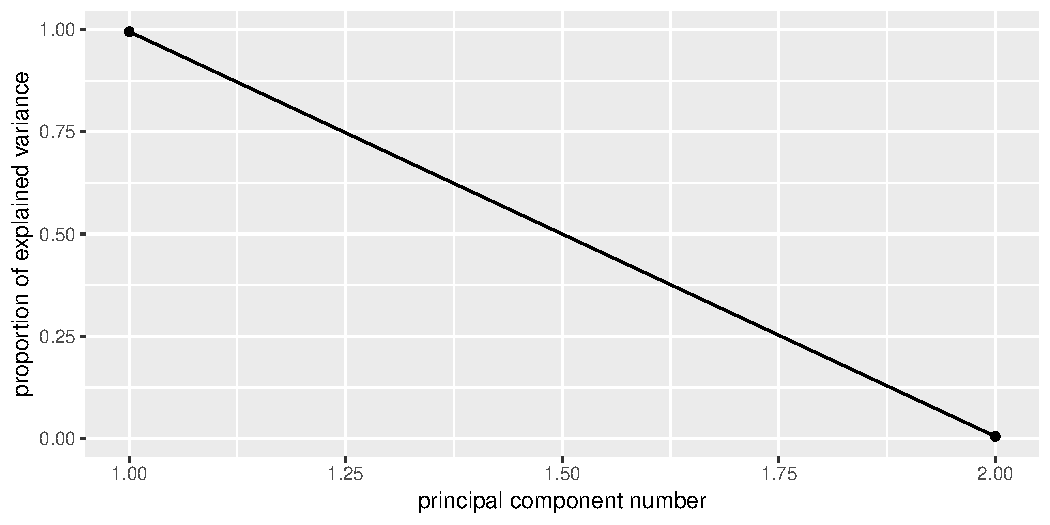
\includegraphics{figure/unnamed-chunk-8-1.pdf}
\caption{plot of chunk unnamed-chunk-8}
\end{figure}

Imagine scree plot continues at zero, so 2 components is a \emph{big}
elbow (take one component).

\end{frame}

\begin{frame}[fragile]{Component loadings}
\protect\hypertarget{component-loadings}{}

explain how each principal component depends on (standardized) original
variables (test scores):

\footnotesize

\begin{Shaded}
\begin{Highlighting}[]
\NormalTok{test12.pc}\OperatorTok{$}\NormalTok{loadings}
\end{Highlighting}
\end{Shaded}

\begin{verbatim}
## 
## Loadings:
##        Comp.1 Comp.2
## first   0.707  0.707
## second  0.707 -0.707
## 
##                Comp.1 Comp.2
## SS loadings       1.0    1.0
## Proportion Var    0.5    0.5
## Cumulative Var    0.5    1.0
\end{verbatim}

\normalsize

First component basically sum of (standardized) test scores. That is,
person tends to score similarly on two tests, and a composite score
would summarize performance.

\end{frame}

\begin{frame}[fragile]{Component scores}
\protect\hypertarget{component-scores}{}

\small

\begin{Shaded}
\begin{Highlighting}[]
\NormalTok{d <-}\StringTok{ }\KeywordTok{data.frame}\NormalTok{(test12, test12.pc}\OperatorTok{$}\NormalTok{scores)}
\NormalTok{d}
\end{Highlighting}
\end{Shaded}

\begin{verbatim}
##   first second id       Comp.1       Comp.2
## 1     2      9  A -2.071819003 -0.146981782
## 2    16     40  B  1.719862811 -0.055762223
## 3     8     17  C -0.762289708  0.207589512
## 4    18     43  D  2.176267535  0.042533250
## 5    10     25  E -0.007460609  0.007460609
## 6     4     10  F -1.734784030  0.070683441
## 7    10     27  G  0.111909141 -0.111909141
## 8    12     30  H  0.568313864 -0.013613668
\end{verbatim}

\normalsize

\begin{itemize}
\item
  Person A is a low scorer, very negative \texttt{comp.1} score.
\item
  Person D is high scorer, high positive \texttt{comp.1} score.
\item
  Person E average scorer, near-zero \texttt{comp.1} score.
\item
  \texttt{comp.2} says basically nothing.
\end{itemize}

\end{frame}

\begin{frame}[fragile]{Plot of scores}
\protect\hypertarget{plot-of-scores}{}

\begin{Shaded}
\begin{Highlighting}[]
\KeywordTok{ggplot}\NormalTok{(d, }\KeywordTok{aes}\NormalTok{(}\DataTypeTok{x =}\NormalTok{ Comp}\FloatTok{.1}\NormalTok{, }\DataTypeTok{y =}\NormalTok{ Comp}\FloatTok{.2}\NormalTok{, }\DataTypeTok{label =}\NormalTok{ id)) }\OperatorTok{+}
\StringTok{  }\KeywordTok{geom_point}\NormalTok{() }\OperatorTok{+}\StringTok{ }\KeywordTok{geom_text_repel}\NormalTok{()}
\end{Highlighting}
\end{Shaded}

\begin{figure}
\centering
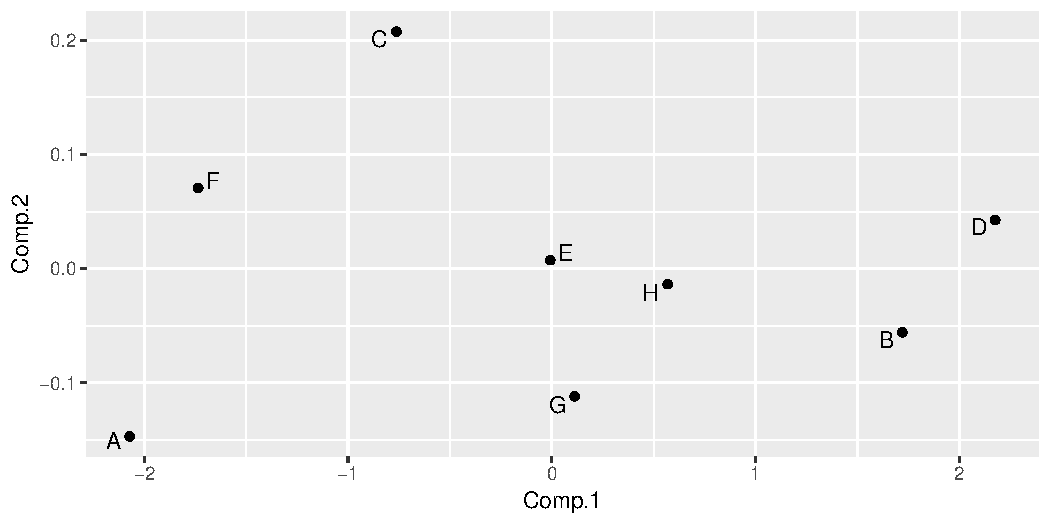
\includegraphics{figure/score-plot-1.pdf}
\caption{plot of chunk score-plot}
\end{figure}

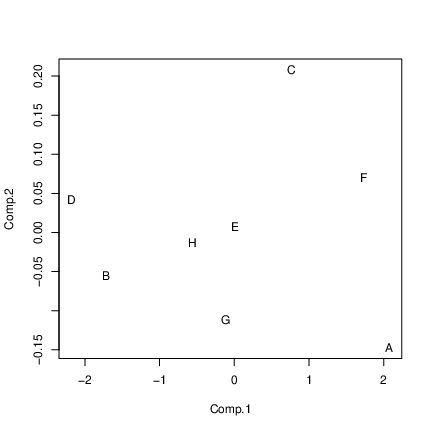
\includegraphics{bPrincomp-score-plot.png}

\end{frame}

\begin{frame}[fragile]{Comments}
\protect\hypertarget{comments-1}{}

\begin{itemize}
\item
  Vertical scale exaggerates importance of \texttt{comp.2}.
\item
  Fix up to get axes on same scale:
\end{itemize}

\begin{Shaded}
\begin{Highlighting}[]
\NormalTok{g <-}\StringTok{ }\KeywordTok{ggplot}\NormalTok{(d, }\KeywordTok{aes}\NormalTok{(}\DataTypeTok{x =}\NormalTok{ Comp}\FloatTok{.1}\NormalTok{, }\DataTypeTok{y =}\NormalTok{ Comp}\FloatTok{.2}\NormalTok{, }\DataTypeTok{label =}\NormalTok{ id)) }\OperatorTok{+}
\StringTok{  }\KeywordTok{geom_point}\NormalTok{() }\OperatorTok{+}\StringTok{ }\KeywordTok{geom_text_repel}\NormalTok{() }\OperatorTok{+}
\StringTok{  }\KeywordTok{coord_fixed}\NormalTok{()}
\end{Highlighting}
\end{Shaded}

\begin{itemize}
\tightlist
\item
  Shows how exam scores really spread out along one dimension:
\end{itemize}

\begin{Shaded}
\begin{Highlighting}[]
\NormalTok{g}
\end{Highlighting}
\end{Shaded}

\begin{figure}
\centering
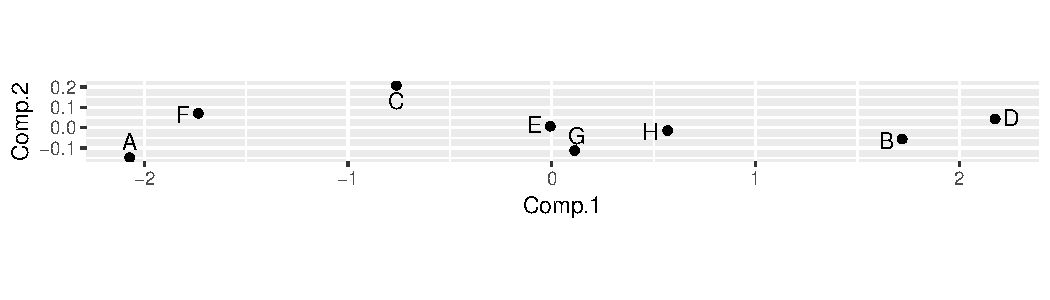
\includegraphics{figure/eqsc2-1.pdf}
\caption{plot of chunk eqsc2}
\end{figure}

\end{frame}

\begin{frame}[fragile]{The biplot}
\protect\hypertarget{the-biplot}{}

\begin{itemize}
\item
  Plotting variables and individuals on one plot.
\item
  Shows how components and original variables related.
\item
  Shows how individuals score on each component, and therefore suggests
  how they score on each variable.
\item
  Add \texttt{labels} option to identify individuals:
\end{itemize}

\begin{Shaded}
\begin{Highlighting}[]
\NormalTok{g <-}\StringTok{ }\KeywordTok{ggbiplot}\NormalTok{(test12.pc, }\DataTypeTok{labels =}\NormalTok{ test12}\OperatorTok{$}\NormalTok{id)}
\end{Highlighting}
\end{Shaded}

\end{frame}

\begin{frame}{The biplot}
\protect\hypertarget{the-biplot-1}{}

\begin{figure}
\centering
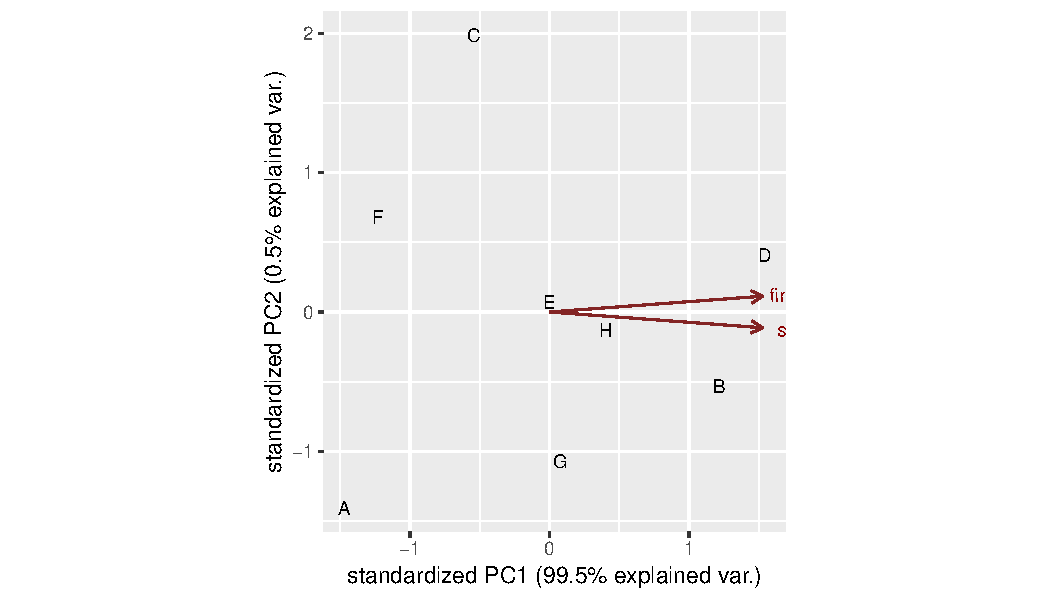
\includegraphics{figure/ff3-1.pdf}
\caption{plot of chunk ff3}
\end{figure}

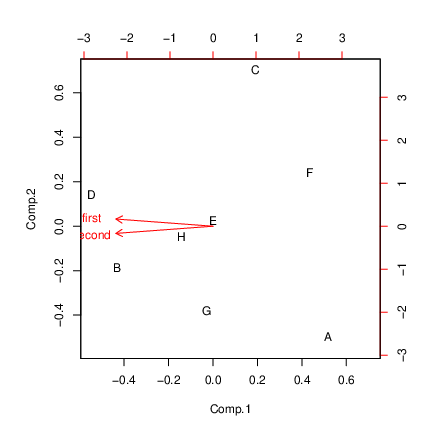
\includegraphics{bPrincomp-test-biplot.png}

\end{frame}

\begin{frame}[fragile]{Comments}
\protect\hypertarget{comments-2}{}

\begin{itemize}
\item
  Variables point almost same direction (left). Thus very negative value
  on \texttt{comp.1} goes with high scores on both tests, and test
  scores highly correlated.
\item
  Position of individuals on plot according to scores on principal
  components, implies values on original variables. Eg.:
\item
  D very negative on \texttt{comp.1}, high scorer on both tests.
\item
  A and F very positive on \texttt{comp.1}, poor scorers on both tests.
\item
  C positive on \texttt{comp.2}, high score on first test relative to
  second.
\item
  A negative on \texttt{comp.2}, high score on second test relative to
  first.
\end{itemize}

\end{frame}

\begin{frame}[fragile]{Track running data}
\protect\hypertarget{track-running-data}{}

Track running records (1984) for distances 100m to marathon, arranged by
country. Countries labelled by (mostly) Internet domain names (ISO
2-letter codes):

\scriptsize

\begin{Shaded}
\begin{Highlighting}[]
\NormalTok{my_url <-}\StringTok{ "http://www.utsc.utoronto.ca/~butler/d29/men_track_field.txt"}
\NormalTok{track <-}\StringTok{ }\KeywordTok{read_table}\NormalTok{(my_url)}
\NormalTok{track }\OperatorTok\StringTok{ }\KeywordTok{sample_n}\NormalTok{(}\DecValTok{10}\NormalTok{)}
\end{Highlighting}
\end{Shaded}

\begin{verbatim}
## # A tibble: 10 x 9
##     m100  m200  m400  m800 m1500 m5000 m10000 marathon country
##    <dbl> <dbl> <dbl> <dbl> <dbl> <dbl>  <dbl>    <dbl> <chr>  
##  1  12.2  23.2  52.9  2.02  4.24  16.7   35.4     165. ck     
##  2  10.2  20.7  46.6  1.78  3.64  14.6   28.4     135. gr     
##  3  10.8  21.9  49    2.02  4.24  16.3   34.7     162. ws     
##  4  10.3  20.9  46.9  1.79  3.77  14.0   29.2     136. kr     
##  5  10.2  20.6  45.6  1.77  3.61  13.3   27.9     131. se     
##  6  10.4  21.3  46.1  1.8   3.65  13.5   28.0     129. mx     
##  7  10.1  20.2  44.9  1.7   3.51  13.0   27.5     129. uk     
##  8  11.0  21.8  47.9  1.9   4.01  14.7   31.4     148. pg     
##  9  10.2  20.2  45.4  1.76  3.6   13.3   27.9     132. pl     
## 10  10.4  20.6  45.6  1.76  3.58  13.4   28.2     134. cz
\end{verbatim}

\normalsize

\end{frame}

\begin{frame}[fragile]{Country names}
\protect\hypertarget{country-names}{}

Also read in a table to look country names up in later:

\footnotesize

\begin{Shaded}
\begin{Highlighting}[]
\NormalTok{my_url <-}\StringTok{ "http://www.utsc.utoronto.ca/~butler/d29/isocodes.csv"}
\NormalTok{iso <-}\StringTok{ }\KeywordTok{read_csv}\NormalTok{(my_url)}
\NormalTok{iso}
\end{Highlighting}
\end{Shaded}

\begin{verbatim}
## # A tibble: 250 x 4
##    Country             ISO2  ISO3    M49
##    <chr>               <chr> <chr> <dbl>
##  1 Afghanistan         af    afg       4
##  2 Aland Islands       ax    ala     248
##  3 Albania             al    alb       8
##  4 Algeria             dz    dza      12
##  5 American Samoa      as    asm      16
##  6 Andorra             ad    and      20
##  7 Angola              ao    ago      24
##  8 Anguilla            ai    aia     660
##  9 Antarctica          aq    ata      10
## 10 Antigua and Barbuda ag    atg      28
## # … with 240 more rows
\end{verbatim}

\normalsize

\end{frame}

\begin{frame}{Data and aims}
\protect\hypertarget{data-and-aims}{}

\begin{itemize}
\item
  Times in seconds 100m--400m, in minutes for rest (800m up).
\item
  This taken care of by standardization.
\item
  8 variables; can we summarize by fewer and gain some insight?
\item
  In particular, if 2 components tell most of story, what do we see in a
  plot?
\end{itemize}

\end{frame}

\begin{frame}[fragile]{Fit and examine principal components}
\protect\hypertarget{fit-and-examine-principal-components}{}

\footnotesize

\begin{Shaded}
\begin{Highlighting}[]
\NormalTok{track }\OperatorTok\StringTok{ }\KeywordTok{select_if}\NormalTok{(is.numeric) ->}\StringTok{ }\NormalTok{track_num}
\NormalTok{track.pc <-}\StringTok{ }\KeywordTok{princomp}\NormalTok{(track_num, }\DataTypeTok{cor =}\NormalTok{ T)}
\KeywordTok{summary}\NormalTok{(track.pc)}
\end{Highlighting}
\end{Shaded}

\begin{verbatim}
## Importance of components:
##                           Comp.1    Comp.2
## Standard deviation     2.5733531 0.9368128
## Proportion of Variance 0.8277683 0.1097023
## Cumulative Proportion  0.8277683 0.9374706
##                            Comp.3     Comp.4
## Standard deviation     0.39915052 0.35220645
## Proportion of Variance 0.01991514 0.01550617
## Cumulative Proportion  0.95738570 0.97289187
##                             Comp.5      Comp.6
## Standard deviation     0.282630981 0.260701267
## Proportion of Variance 0.009985034 0.008495644
## Cumulative Proportion  0.982876903 0.991372547
##                             Comp.7      Comp.8
## Standard deviation     0.215451919 0.150333291
## Proportion of Variance 0.005802441 0.002825012
## Cumulative Proportion  0.997174988 1.000000000
\end{verbatim}

\normalsize

\end{frame}

\begin{frame}[fragile]{Scree plot}
\protect\hypertarget{scree-plot-1}{}

\begin{Shaded}
\begin{Highlighting}[]
\KeywordTok{ggscreeplot}\NormalTok{(track.pc)}
\end{Highlighting}
\end{Shaded}

\begin{figure}
\centering
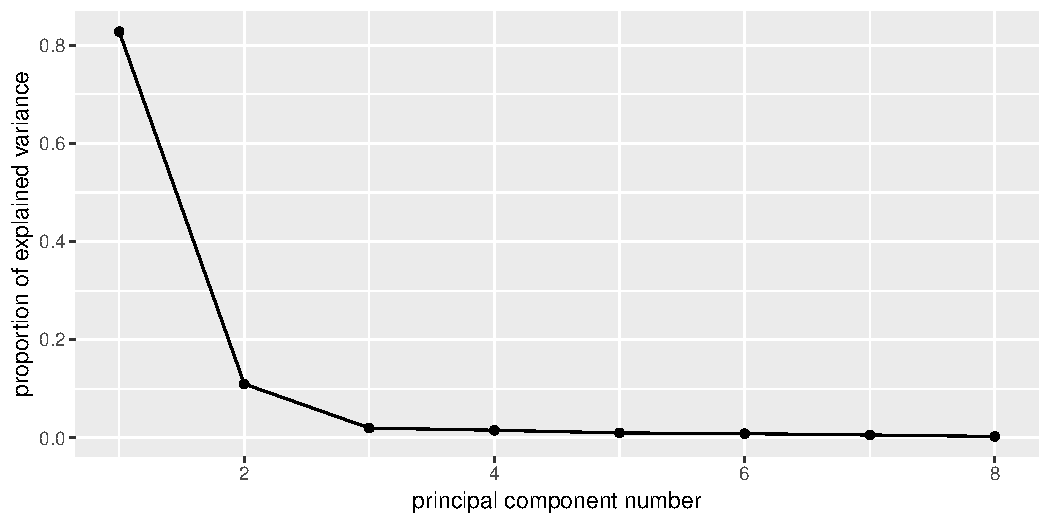
\includegraphics{figure/scree-b-1.pdf}
\caption{plot of chunk scree-b}
\end{figure}

\end{frame}

\begin{frame}[fragile]{How many components?}
\protect\hypertarget{how-many-components}{}

\begin{itemize}
\item
  As for discriminant analysis, look for ``elbow'' in scree plot.
\item
  See one here at 3 components; everything 3 and beyond is ``scree''.
\item
  So take 2 components.
\item
  Note difference from discriminant analysis: want ``large'' rather than
  ``small'', so go 1 step left of elbow.
\item
  Another criterion: any component with eigenvalue bigger than about 1
  is worth including. 2nd one here has eigenvalue just less than 1.
\item
  Refer back to \texttt{summary}: cumulative proportion of variance
  explained for 2 components is 93.7\%, pleasantly high. 2 components
  tell almost whole story.
\end{itemize}

\end{frame}

\begin{frame}[fragile]{How do components depend on original variables?}
\protect\hypertarget{how-do-components-depend-on-original-variables}{}

Loadings:

\footnotesize

\begin{Shaded}
\begin{Highlighting}[]
\NormalTok{track.pc}\OperatorTok{$}\NormalTok{loadings}
\end{Highlighting}
\end{Shaded}

\begin{verbatim}
## 
## Loadings:
##          Comp.1 Comp.2 Comp.3 Comp.4 Comp.5 Comp.6 Comp.7 Comp.8
## m100      0.318  0.567  0.332  0.128  0.263  0.594  0.136  0.106
## m200      0.337  0.462  0.361 -0.259 -0.154 -0.656 -0.113       
## m400      0.356  0.248 -0.560  0.652 -0.218 -0.157              
## m800      0.369        -0.532 -0.480  0.540        -0.238       
## m1500     0.373 -0.140 -0.153 -0.405 -0.488  0.158  0.610  0.139
## m5000     0.364 -0.312  0.190        -0.254  0.141 -0.591  0.547
## m10000    0.367 -0.307  0.182        -0.133  0.219 -0.177 -0.797
## marathon  0.342 -0.439  0.263  0.300  0.498 -0.315  0.399  0.158
## 
##                Comp.1 Comp.2 Comp.3 Comp.4 Comp.5 Comp.6 Comp.7
## SS loadings     1.000  1.000  1.000  1.000  1.000  1.000  1.000
## Proportion Var  0.125  0.125  0.125  0.125  0.125  0.125  0.125
## Cumulative Var  0.125  0.250  0.375  0.500  0.625  0.750  0.875
##                Comp.8
## SS loadings     1.000
## Proportion Var  0.125
## Cumulative Var  1.000
\end{verbatim}

\normalsize

\end{frame}

\begin{frame}[fragile]{Comments}
\protect\hypertarget{comments-3}{}

\begin{itemize}
\item
  \texttt{comp.1} loads about equally (has equal weight) on times over
  all distances.
\item
  \texttt{comp.2} has large positive loading for short distances, large
  negative for long ones.
\item
  \texttt{comp.3}: large negative for middle distance, large positive
  especially for short distances.
\item
  Country overall good at running will have lower than average record
  times at all distances, so \texttt{comp.1} \emph{small}. Conversely,
  for countries bad at running, \texttt{comp.1} very positive.
\item
  Countries relatively better at sprinting (low times) will be
  \emph{negative} on \texttt{comp.2}; countries relatively better at
  distance running \emph{positive} on \texttt{comp.2}.
\end{itemize}

\end{frame}

\begin{frame}[fragile]{Commands for plots}
\protect\hypertarget{commands-for-plots}{}

\begin{itemize}
\tightlist
\item
  Principal component scores (first two). Also need country IDs.
\end{itemize}

\begin{Shaded}
\begin{Highlighting}[]
\NormalTok{d <-}\StringTok{ }\KeywordTok{data.frame}\NormalTok{(track.pc}\OperatorTok{$}\NormalTok{scores,}
  \DataTypeTok{country =}\NormalTok{ track}\OperatorTok{$}\NormalTok{country}
\NormalTok{)}
\KeywordTok{names}\NormalTok{(d)}
\end{Highlighting}
\end{Shaded}

\begin{verbatim}
## [1] "Comp.1"  "Comp.2"  "Comp.3"  "Comp.4"  "Comp.5"  "Comp.6" 
## [7] "Comp.7"  "Comp.8"  "country"
\end{verbatim}

\begin{Shaded}
\begin{Highlighting}[]
\NormalTok{g1 <-}\StringTok{ }\KeywordTok{ggplot}\NormalTok{(d, }\KeywordTok{aes}\NormalTok{(}\DataTypeTok{x =}\NormalTok{ Comp}\FloatTok{.1}\NormalTok{, }\DataTypeTok{y =}\NormalTok{ Comp}\FloatTok{.2}\NormalTok{,}
  \DataTypeTok{label =}\NormalTok{ country)) }\OperatorTok{+}
\StringTok{  }\KeywordTok{geom_point}\NormalTok{() }\OperatorTok{+}\StringTok{ }\KeywordTok{geom_text_repel}\NormalTok{() }\OperatorTok{+}\StringTok{ }\KeywordTok{coord_fixed}\NormalTok{()}
\end{Highlighting}
\end{Shaded}

\begin{itemize}
\tightlist
\item
  Biplot:
\end{itemize}

\begin{Shaded}
\begin{Highlighting}[]
\NormalTok{g2 <-}\StringTok{ }\KeywordTok{ggbiplot}\NormalTok{(track.pc, }\DataTypeTok{labels =}\NormalTok{ track}\OperatorTok{$}\NormalTok{country)}
\end{Highlighting}
\end{Shaded}

\end{frame}

\begin{frame}[fragile]{Principal components plot}
\protect\hypertarget{principal-components-plot}{}

\begin{Shaded}
\begin{Highlighting}[]
\NormalTok{g1}
\end{Highlighting}
\end{Shaded}

\begin{figure}
\centering
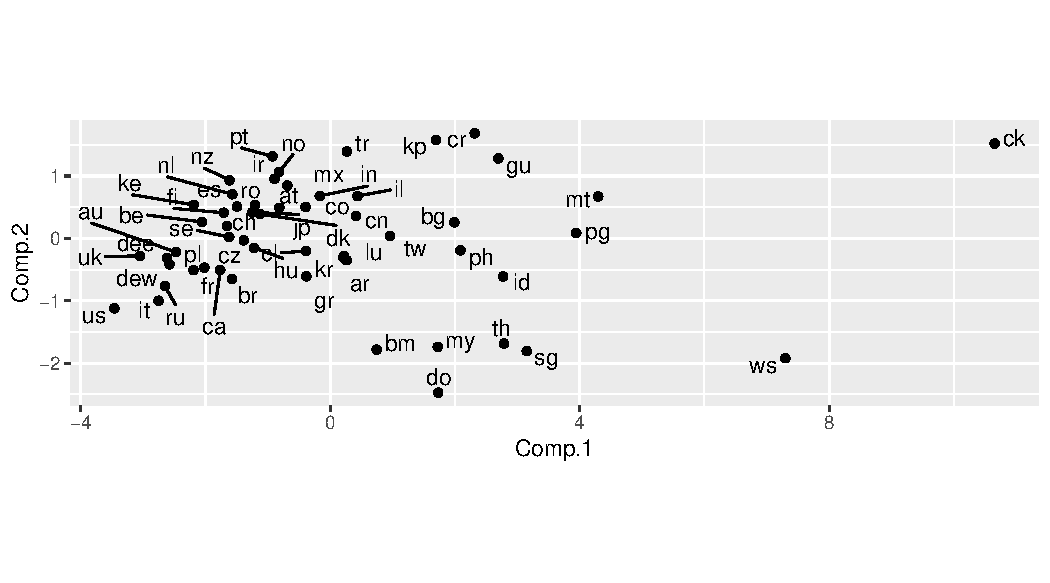
\includegraphics{figure/lecce-1.pdf}
\caption{plot of chunk lecce}
\end{figure}

\end{frame}

\begin{frame}[fragile]{Comments on principal components plot}
\protect\hypertarget{comments-on-principal-components-plot}{}

\begin{itemize}
\item
  Good running countries at left of plot: US, UK, Italy, Russia, East
  and West Germany.
\item
  Bad running countries at right: Western Samoa, Cook Islands.
\item
  Better sprinting countries at bottom: US, Italy, Russia, Brazil,
  Greece. \texttt{do} is Dominican Republic, where sprinting records
  relatively good, distance records very bad.
\item
  Better distance-running countries at top: Portugal, Norway, Turkey,
  Ireland, New Zealand, Mexico. \texttt{ke} is Kenya.
\end{itemize}

\end{frame}

\begin{frame}[fragile]{Biplot}
\protect\hypertarget{biplot}{}

\begin{Shaded}
\begin{Highlighting}[]
\NormalTok{g2}
\end{Highlighting}
\end{Shaded}

\begin{figure}
\centering
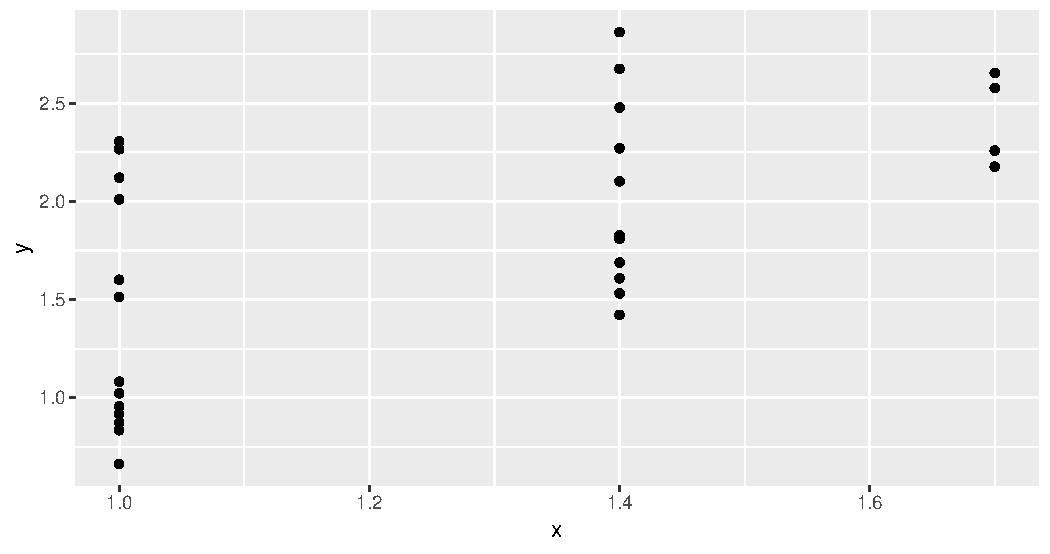
\includegraphics{figure/biplot2-1.pdf}
\caption{plot of chunk biplot2}
\end{figure}

\end{frame}

\begin{frame}{Comments on biplot}
\protect\hypertarget{comments-on-biplot}{}

\begin{itemize}
\item
  Had to do some pre-work to interpret PC plot. Biplot more
  self-contained.
\item
  All variable arrows point right; countries on right have large (bad)
  record times overall, countries on left good overall.
\item
  Imagine that variable arrows extend negatively as well. Bottom right =
  bad at distance running, top left = good at distance running.
\item
  Top right = bad at sprinting, bottom left = good at sprinting.
\item
  Doesn't require so much pre-interpretation of components.
\end{itemize}

\end{frame}

\begin{frame}[fragile]{Best 8 running countries}
\protect\hypertarget{best-8-running-countries}{}

Need to look up two-letter abbreviations in ISO table:

\footnotesize

\begin{Shaded}
\begin{Highlighting}[]
\NormalTok{d }\OperatorTok
\StringTok{  }\KeywordTok{arrange}\NormalTok{(Comp}\FloatTok{.1}\NormalTok{) }\OperatorTok
\StringTok{  }\KeywordTok{left_join}\NormalTok{(iso, }\DataTypeTok{by =} \KeywordTok{c}\NormalTok{(}\StringTok{"country"}\NormalTok{ =}\StringTok{ "ISO2"}\NormalTok{)) }\OperatorTok
\StringTok{  }\KeywordTok{select}\NormalTok{(Comp}\FloatTok{.1}\NormalTok{, country, Country) }\OperatorTok
\StringTok{  }\KeywordTok{slice}\NormalTok{(}\DecValTok{1}\OperatorTok{:}\DecValTok{8}\NormalTok{)}
\end{Highlighting}
\end{Shaded}

\begin{verbatim}
##      Comp.1 country                  Country
## 1 -3.462175      us United States of America
## 2 -3.052104      uk           United Kingdom
## 3 -2.752084      it                    Italy
## 4 -2.651062      ru       Russian Federation
## 5 -2.613964     dee             East Germany
## 6 -2.576272     dew             West Germany
## 7 -2.468919      au                Australia
## 8 -2.191917      fr                   France
\end{verbatim}

\normalsize

\end{frame}

\begin{frame}[fragile]{Worst 8 running countries}
\protect\hypertarget{worst-8-running-countries}{}

\footnotesize

\begin{Shaded}
\begin{Highlighting}[]
\NormalTok{d }\OperatorTok
\StringTok{  }\KeywordTok{arrange}\NormalTok{(}\KeywordTok{desc}\NormalTok{(Comp}\FloatTok{.1}\NormalTok{)) }\OperatorTok
\StringTok{  }\KeywordTok{left_join}\NormalTok{(iso, }\DataTypeTok{by =} \KeywordTok{c}\NormalTok{(}\StringTok{"country"}\NormalTok{ =}\StringTok{ "ISO2"}\NormalTok{)) }\OperatorTok
\StringTok{  }\KeywordTok{select}\NormalTok{(Comp}\FloatTok{.1}\NormalTok{, country, Country) }\OperatorTok
\StringTok{  }\KeywordTok{slice}\NormalTok{(}\DecValTok{1}\OperatorTok{:}\DecValTok{8}\NormalTok{)}
\end{Highlighting}
\end{Shaded}

\begin{verbatim}
##      Comp.1 country          Country
## 1 10.652914      ck     Cook Islands
## 2  7.297865      ws            Samoa
## 3  4.297909      mt            Malta
## 4  3.945224      pg Papua New Guinea
## 5  3.150886      sg        Singapore
## 6  2.787273      th         Thailand
## 7  2.773125      id        Indonesia
## 8  2.697066      gu             Guam
\end{verbatim}

\normalsize

\end{frame}

\begin{frame}[fragile]{Better at distance running}
\protect\hypertarget{better-at-distance-running}{}

\footnotesize

\begin{Shaded}
\begin{Highlighting}[]
\NormalTok{d }\OperatorTok
\StringTok{  }\KeywordTok{arrange}\NormalTok{(}\KeywordTok{desc}\NormalTok{(Comp}\FloatTok{.2}\NormalTok{)) }\OperatorTok
\StringTok{  }\KeywordTok{left_join}\NormalTok{(iso, }\DataTypeTok{by =} \KeywordTok{c}\NormalTok{(}\StringTok{"country"}\NormalTok{ =}\StringTok{ "ISO2"}\NormalTok{)) }\OperatorTok
\StringTok{  }\KeywordTok{select}\NormalTok{(Comp}\FloatTok{.2}\NormalTok{, country, Country) }\OperatorTok
\StringTok{  }\KeywordTok{slice}\NormalTok{(}\DecValTok{1}\OperatorTok{:}\DecValTok{10}\NormalTok{)}
\end{Highlighting}
\end{Shaded}

\begin{verbatim}
##       Comp.2 country                   Country
## 1  1.6860391      cr                Costa Rica
## 2  1.5791490      kp             Korea (North)
## 3  1.5226742      ck              Cook Islands
## 4  1.3957839      tr                    Turkey
## 5  1.3167578      pt                  Portugal
## 6  1.2829272      gu                      Guam
## 7  1.0663756      no                    Norway
## 8  0.9547437      ir Iran, Islamic Republic of
## 9  0.9318729      nz               New Zealand
## 10 0.8495104      mx                    Mexico
\end{verbatim}

\normalsize

\end{frame}

\begin{frame}[fragile]{Better at sprinting}
\protect\hypertarget{better-at-sprinting}{}

\footnotesize

\begin{Shaded}
\begin{Highlighting}[]
\NormalTok{d }\OperatorTok
\StringTok{  }\KeywordTok{arrange}\NormalTok{(Comp}\FloatTok{.2}\NormalTok{) }\OperatorTok
\StringTok{  }\KeywordTok{left_join}\NormalTok{(iso, }\DataTypeTok{by =} \KeywordTok{c}\NormalTok{(}\StringTok{"country"}\NormalTok{ =}\StringTok{ "ISO2"}\NormalTok{)) }\OperatorTok
\StringTok{  }\KeywordTok{select}\NormalTok{(Comp}\FloatTok{.2}\NormalTok{, country, Country) }\OperatorTok
\StringTok{  }\KeywordTok{slice}\NormalTok{(}\DecValTok{1}\OperatorTok{:}\DecValTok{10}\NormalTok{)}
\end{Highlighting}
\end{Shaded}

\begin{verbatim}
##        Comp.2 country                  Country
## 1  -2.4715736      do       Dominican Republic
## 2  -1.9196130      ws                    Samoa
## 3  -1.8055052      sg                Singapore
## 4  -1.7832229      bm                  Bermuda
## 5  -1.7386063      my                 Malaysia
## 6  -1.6851772      th                 Thailand
## 7  -1.1204235      us United States of America
## 8  -0.9989821      it                    Italy
## 9  -0.7639385      ru       Russian Federation
## 10 -0.6470634      br                   Brazil
\end{verbatim}

\normalsize

\end{frame}

\begin{frame}[fragile]{Plot with country names}
\protect\hypertarget{plot-with-country-names}{}

\begin{Shaded}
\begin{Highlighting}[]
\NormalTok{g <-}\StringTok{ }\NormalTok{d }\OperatorTok
\StringTok{  }\KeywordTok{left_join}\NormalTok{(iso, }\DataTypeTok{by =} \KeywordTok{c}\NormalTok{(}\StringTok{"country"}\NormalTok{ =}\StringTok{ "ISO2"}\NormalTok{)) }\OperatorTok
\StringTok{  }\KeywordTok{select}\NormalTok{(Comp}\FloatTok{.1}\NormalTok{, Comp}\FloatTok{.2}\NormalTok{, Country) }\OperatorTok
\StringTok{  }\KeywordTok{ggplot}\NormalTok{(}\KeywordTok{aes}\NormalTok{(}\DataTypeTok{x =}\NormalTok{ Comp}\FloatTok{.1}\NormalTok{, }\DataTypeTok{y =}\NormalTok{ Comp}\FloatTok{.2}\NormalTok{, }\DataTypeTok{label =}\NormalTok{ Country)) }\OperatorTok{+}
\StringTok{  }\KeywordTok{geom_point}\NormalTok{() }\OperatorTok{+}\StringTok{ }\KeywordTok{geom_text_repel}\NormalTok{(}\DataTypeTok{size =} \DecValTok{1}\NormalTok{) }\OperatorTok{+}
\StringTok{  }\KeywordTok{coord_fixed}\NormalTok{()}
\end{Highlighting}
\end{Shaded}

\begin{verbatim}
## Warning: Column `country`/`ISO2` joining factor and character
## vector, coercing into character vector
\end{verbatim}

\end{frame}

\begin{frame}[fragile]{The plot}
\protect\hypertarget{the-plot-1}{}

\begin{Shaded}
\begin{Highlighting}[]
\NormalTok{g}
\end{Highlighting}
\end{Shaded}

\begin{figure}
\centering
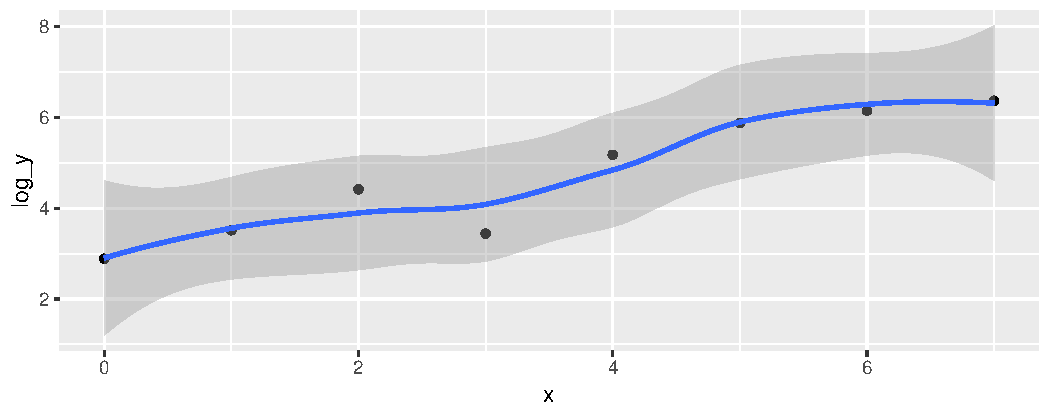
\includegraphics{figure/unnamed-chunk-22-1.pdf}
\caption{plot of chunk unnamed-chunk-22}
\end{figure}

\end{frame}

\begin{frame}[fragile]{Principal components from correlation matrix}
\protect\hypertarget{principal-components-from-correlation-matrix}{}

Create data file like this:

\begin{verbatim}
 1        0.9705 -0.9600
 0.9705   1      -0.9980
-0.9600  -0.9980  1
\end{verbatim}

and read in like this:

\begin{Shaded}
\begin{Highlighting}[]
\NormalTok{my_url <-}\StringTok{ "http://www.utsc.utoronto.ca/~butler/d29/cov.txt"}
\NormalTok{mat <-}\StringTok{ }\KeywordTok{read_table}\NormalTok{(my_url, }\DataTypeTok{col_names =}\NormalTok{ F)}
\NormalTok{mat}
\end{Highlighting}
\end{Shaded}

\begin{verbatim}
## # A tibble: 3 x 3
##       X1     X2     X3
##    <dbl>  <dbl>  <dbl>
## 1  1      0.970 -0.96 
## 2  0.970  1     -0.998
## 3 -0.96  -0.998  1
\end{verbatim}

\end{frame}

\begin{frame}[fragile]{Pre-processing}
\protect\hypertarget{pre-processing}{}

A little pre-processing required:

\begin{itemize}
\item
  Turn into matrix (from data frame)
\item
  Feed into \texttt{princomp} as \texttt{covmat=}
\end{itemize}

\begin{Shaded}
\begin{Highlighting}[]
\NormalTok{mat.pc <-}\StringTok{ }\NormalTok{mat }\OperatorTok
\StringTok{  }\KeywordTok{as.matrix}\NormalTok{() }\OperatorTok
\StringTok{  }\KeywordTok{princomp}\NormalTok{(}\DataTypeTok{covmat =}\NormalTok{ .)}
\end{Highlighting}
\end{Shaded}

\end{frame}

\begin{frame}[fragile]{Scree plot: one component fine}
\protect\hypertarget{scree-plot-one-component-fine}{}

\begin{Shaded}
\begin{Highlighting}[]
\KeywordTok{ggscreeplot}\NormalTok{(mat.pc)}
\end{Highlighting}
\end{Shaded}

\begin{figure}
\centering
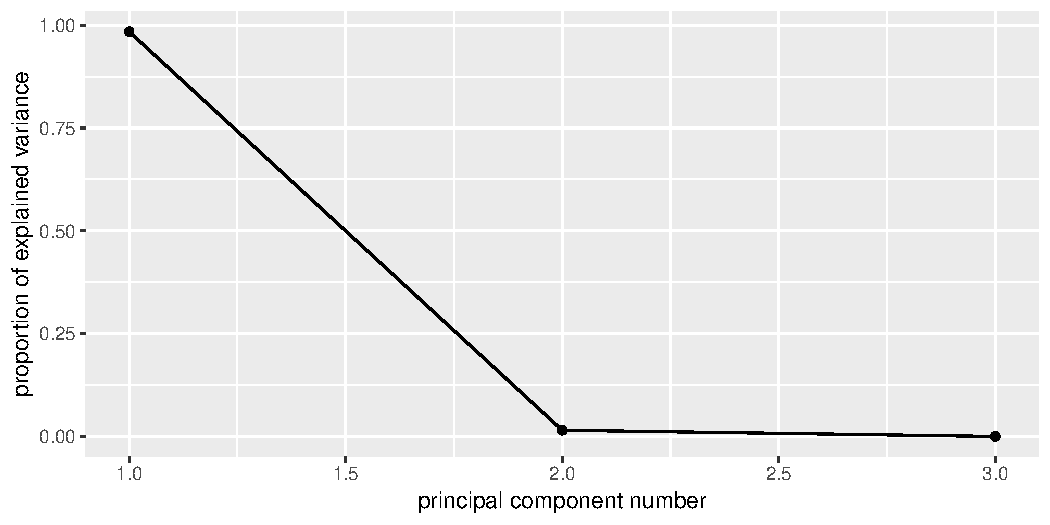
\includegraphics{figure/palermo-1.pdf}
\caption{plot of chunk palermo}
\end{figure}

\end{frame}

\begin{frame}[fragile]{Component loadings}
\protect\hypertarget{component-loadings-1}{}

Compare correlation matrix:

\scriptsize

\begin{Shaded}
\begin{Highlighting}[]
\NormalTok{mat}
\end{Highlighting}
\end{Shaded}

\begin{verbatim}
## # A tibble: 3 x 3
##       X1     X2     X3
##    <dbl>  <dbl>  <dbl>
## 1  1      0.970 -0.96 
## 2  0.970  1     -0.998
## 3 -0.96  -0.998  1
\end{verbatim}

\normalsize

with component loadings

\scriptsize

\begin{Shaded}
\begin{Highlighting}[]
\NormalTok{mat.pc}\OperatorTok{$}\NormalTok{loadings}
\end{Highlighting}
\end{Shaded}

\begin{verbatim}
## 
## Loadings:
##    Comp.1 Comp.2 Comp.3
## X1  0.573  0.812  0.112
## X2  0.581 -0.306 -0.755
## X3 -0.578  0.498 -0.646
## 
##                Comp.1 Comp.2 Comp.3
## SS loadings     1.000  1.000  1.000
## Proportion Var  0.333  0.333  0.333
## Cumulative Var  0.333  0.667  1.000
\end{verbatim}

\normalsize

\end{frame}

\begin{frame}[fragile]{Comments}
\protect\hypertarget{comments-4}{}

\begin{itemize}
\item
  When X1 large, X2 also large, X3 small.

  \begin{itemize}
  \tightlist
  \item
    Then \texttt{comp.1} \emph{positive}.
  \end{itemize}
\item
  When X1 small, X2 small, X3 large.

  \begin{itemize}
  \tightlist
  \item
    Then \texttt{comp.1} \emph{negative}.
  \end{itemize}
\end{itemize}

\end{frame}

\begin{frame}{No scores}
\protect\hypertarget{no-scores}{}

\begin{itemize}
\item
  With correlation matrix rather than data, no component scores

  \begin{itemize}
  \item
    So no principal component plot
  \item
    and no biplot.
  \end{itemize}
\end{itemize}

\end{frame}

\hypertarget{exploratory-factor-analysis}{%
\section{Exploratory factor
analysis}\label{exploratory-factor-analysis}}

\begin{frame}{Principal components and factor analysis}
\protect\hypertarget{principal-components-and-factor-analysis}{}

\begin{itemize}
\item
  Principal components:

  \begin{itemize}
  \item
    Purely mathematical.
  \item
    Find eigenvalues, eigenvectors of correlation matrix.
  \item
    No testing whether observed components reproducible, or even
    probability model behind it.
  \end{itemize}
\item
  Factor analysis:

  \begin{itemize}
  \item
    some way towards fixing this (get test of appropriateness)
  \item
    In factor analysis, each variable modelled as: ``common factor''
    (eg. verbal ability) and ``specific factor'' (left over).
  \item
    Choose the common factors to ``best'' reproduce pattern seen in
    correlation matrix.
  \item
    Iterative procedure, different answer from principal components.
  \end{itemize}
\end{itemize}

\end{frame}

\begin{frame}[fragile]{Packages}
\protect\hypertarget{packages-1}{}

\begin{Shaded}
\begin{Highlighting}[]
\KeywordTok{library}\NormalTok{(lavaan) }\CommentTok{# for confirmatory, later}
\KeywordTok{library}\NormalTok{(ggbiplot)}
\KeywordTok{library}\NormalTok{(tidyverse)}
\end{Highlighting}
\end{Shaded}

\end{frame}

\begin{frame}[fragile]{Example}
\protect\hypertarget{example}{}

\begin{itemize}
\item
  145 children given 5 tests, called PARA, SENT, WORD, ADD and DOTS. 3
  linguistic tasks (paragraph comprehension, sentence completion and
  word meaning), 2 mathematical ones (addition and counting dots).
\item
  Correlation matrix of scores on the tests:
\end{itemize}

\begin{verbatim}

para 1     0.722 0.714 0.203 0.095
sent 0.722 1     0.685 0.246 0.181
word 0.714 0.685 1     0.170 0.113
add  0.203 0.246 0.170 1     0.585
dots 0.095 0.181 0.113 0.585 1
\end{verbatim}

\begin{itemize}
\tightlist
\item
  Is there small number of underlying ``constructs'' (unobservable) that
  explains this pattern of correlations?
\end{itemize}

\end{frame}

\begin{frame}[fragile]{To start: principal components}
\protect\hypertarget{to-start-principal-components}{}

Using correlation matrix. Read that first:

\begin{Shaded}
\begin{Highlighting}[]
\NormalTok{my_url <-}\StringTok{ "http://www.utsc.utoronto.ca/~butler/d29/rex2.txt"}
\NormalTok{kids <-}\StringTok{ }\KeywordTok{read_delim}\NormalTok{(my_url, }\StringTok{" "}\NormalTok{)}
\NormalTok{kids}
\end{Highlighting}
\end{Shaded}

\begin{verbatim}
## # A tibble: 5 x 6
##   test   para  sent  word   add  dots
##   <chr> <dbl> <dbl> <dbl> <dbl> <dbl>
## 1 para  1     0.722 0.714 0.203 0.095
## 2 sent  0.722 1     0.685 0.246 0.181
## 3 word  0.714 0.685 1     0.17  0.113
## 4 add   0.203 0.246 0.17  1     0.585
## 5 dots  0.095 0.181 0.113 0.585 1
\end{verbatim}

\end{frame}

\begin{frame}[fragile]{Principal components on correlation matrix}
\protect\hypertarget{principal-components-on-correlation-matrix}{}

\begin{Shaded}
\begin{Highlighting}[]
\NormalTok{kids }\OperatorTok
\StringTok{  }\KeywordTok{select_if}\NormalTok{(is.numeric) }\OperatorTok
\StringTok{  }\KeywordTok{as.matrix}\NormalTok{() }\OperatorTok
\StringTok{  }\KeywordTok{princomp}\NormalTok{(}\DataTypeTok{covmat =}\NormalTok{ .) ->}\StringTok{ }\NormalTok{kids.pc}
\end{Highlighting}
\end{Shaded}

\end{frame}

\begin{frame}[fragile]{Scree plot}
\protect\hypertarget{scree-plot-2}{}

\begin{Shaded}
\begin{Highlighting}[]
\KeywordTok{ggscreeplot}\NormalTok{(kids.pc)}
\end{Highlighting}
\end{Shaded}

\begin{figure}
\centering
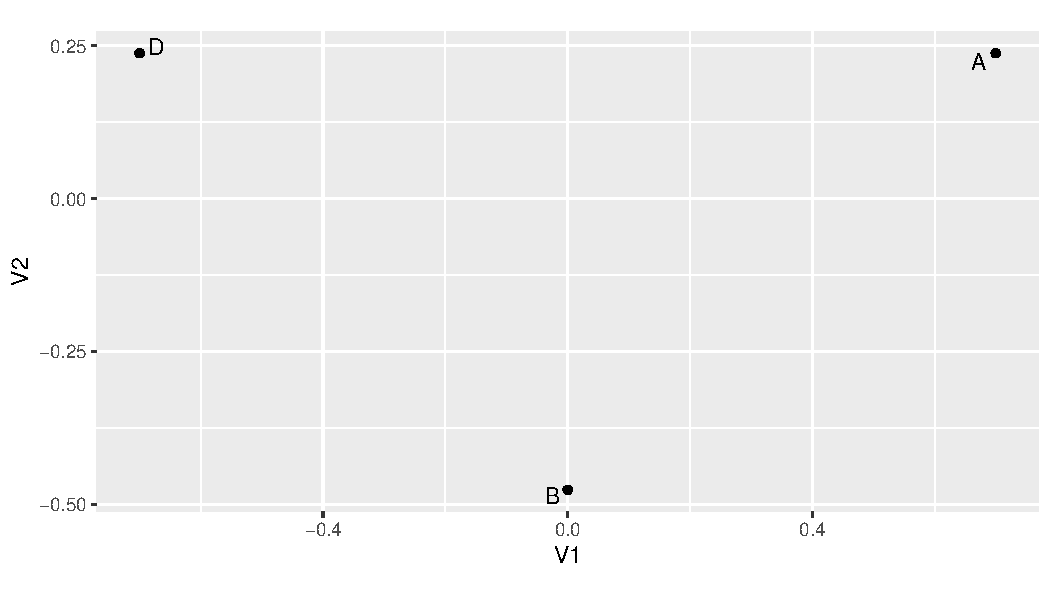
\includegraphics{figure/unnamed-chunk-28-1.pdf}
\caption{plot of chunk unnamed-chunk-28}
\end{figure}

\end{frame}

\begin{frame}[fragile]{Principal component results}
\protect\hypertarget{principal-component-results}{}

\begin{itemize}
\tightlist
\item
  Need 2 components. Loadings:
\end{itemize}

\footnotesize

\begin{Shaded}
\begin{Highlighting}[]
\NormalTok{kids.pc}\OperatorTok{$}\NormalTok{loadings}
\end{Highlighting}
\end{Shaded}

\begin{verbatim}
## 
## Loadings:
##      Comp.1 Comp.2 Comp.3 Comp.4 Comp.5
## para  0.534  0.245  0.114         0.795
## sent  0.542  0.164         0.660 -0.489
## word  0.523  0.247 -0.144 -0.738 -0.316
## add   0.297 -0.627  0.707              
## dots  0.241 -0.678 -0.680         0.143
## 
##                Comp.1 Comp.2 Comp.3 Comp.4 Comp.5
## SS loadings       1.0    1.0    1.0    1.0    1.0
## Proportion Var    0.2    0.2    0.2    0.2    0.2
## Cumulative Var    0.2    0.4    0.6    0.8    1.0
\end{verbatim}

\normalsize

\end{frame}

\begin{frame}[fragile]{Comments}
\protect\hypertarget{comments-5}{}

\begin{itemize}
\item
  First component has a bit of everything, though especially the first
  three tests.
\item
  Second component rather more clearly \texttt{add} and \texttt{dots}.
\item
  No scores, plots since no actual data.
\end{itemize}

\end{frame}

\begin{frame}[fragile]{Factor analysis}
\protect\hypertarget{factor-analysis}{}

\begin{itemize}
\item
  Specify number of factors first, get solution with exactly that many
  factors.
\item
  Includes hypothesis test, need to specify how many children wrote the
  tests.
\item
  Works from correlation matrix via \texttt{covmat} or actual data, like
  \texttt{princomp}.
\item
  Introduces extra feature, \emph{rotation}, to make interpretation of
  loadings (factor-variable relation) easier.
\end{itemize}

\end{frame}

\begin{frame}[fragile]{Factor analysis for the kids data}
\protect\hypertarget{factor-analysis-for-the-kids-data}{}

\begin{itemize}
\item
  Create ``covariance list'' to include number of children who wrote the
  tests.
\item
  Feed this into \texttt{factanal}, specifying how many factors (2).
\end{itemize}

\begin{Shaded}
\begin{Highlighting}[]
\NormalTok{km <-}\StringTok{ }\NormalTok{kids }\OperatorTok
\StringTok{  }\KeywordTok{select_if}\NormalTok{(is.numeric) }\OperatorTok
\StringTok{  }\KeywordTok{as.matrix}\NormalTok{()}
\NormalTok{km2 <-}\StringTok{ }\KeywordTok{list}\NormalTok{(}\DataTypeTok{cov =}\NormalTok{ km, }\DataTypeTok{n.obs =} \DecValTok{145}\NormalTok{)}
\NormalTok{kids.f2 <-}\StringTok{ }\KeywordTok{factanal}\NormalTok{(}\DataTypeTok{factors =} \DecValTok{2}\NormalTok{, }\DataTypeTok{covmat =}\NormalTok{ km2)}
\end{Highlighting}
\end{Shaded}

\end{frame}

\begin{frame}[fragile]{Uniquenesses}
\protect\hypertarget{uniquenesses}{}

\begin{Shaded}
\begin{Highlighting}[]
\NormalTok{kids.f2}\OperatorTok{$}\NormalTok{uniquenesses}
\end{Highlighting}
\end{Shaded}

\begin{verbatim}
##      para      sent      word       add      dots 
## 0.2424457 0.2997349 0.3272312 0.5743568 0.1554076
\end{verbatim}

\begin{itemize}
\item
  Uniquenesses say how ``unique'' a variable is (size of specific
  factor). Small uniqueness means that the variable is summarized by a
  factor (good).
\item
  Very large uniquenesses are bad; \texttt{add}'s uniqueness is largest
  but not large enough to be worried about.
\item
  Also see ``communality'' for this idea, where \emph{large} is good and
  \emph{small} is bad.
\end{itemize}

\end{frame}

\begin{frame}[fragile]{Loadings}
\protect\hypertarget{loadings}{}

\footnotesize

\begin{Shaded}
\begin{Highlighting}[]
\NormalTok{kids.f2}\OperatorTok{$}\NormalTok{loadings}
\end{Highlighting}
\end{Shaded}

\begin{verbatim}
## 
## Loadings:
##      Factor1 Factor2
## [1,] 0.867          
## [2,] 0.820   0.166  
## [3,] 0.816          
## [4,] 0.167   0.631  
## [5,]         0.918  
## 
##                Factor1 Factor2
## SS loadings      2.119   1.282
## Proportion Var   0.424   0.256
## Cumulative Var   0.424   0.680
\end{verbatim}

\normalsize

\begin{itemize}
\tightlist
\item
  Loadings show how each factor depends on variables. Blanks indicate
  ``small'', less than 0.1.
\end{itemize}

\end{frame}

\begin{frame}{Comments}
\protect\hypertarget{comments-6}{}

\begin{itemize}
\item
  Factor 1 clearly the ``linguistic'' tasks, factor 2 clearly the
  ``mathematical'' ones.
\item
  Two factors together explain 68\% of variability (like regression
  R-squared).
\item
  Which variables belong to which factor is \emph{much} clearer than
  with principal components.
\end{itemize}

\end{frame}

\begin{frame}[fragile]{Are 2 factors enough?}
\protect\hypertarget{are-2-factors-enough}{}

\begin{Shaded}
\begin{Highlighting}[]
\NormalTok{kids.f2}\OperatorTok{$}\NormalTok{STATISTIC}
\end{Highlighting}
\end{Shaded}

\begin{verbatim}
## objective 
## 0.5810578
\end{verbatim}

\begin{Shaded}
\begin{Highlighting}[]
\NormalTok{kids.f2}\OperatorTok{$}\NormalTok{dof}
\end{Highlighting}
\end{Shaded}

\begin{verbatim}
## [1] 1
\end{verbatim}

\begin{Shaded}
\begin{Highlighting}[]
\NormalTok{kids.f2}\OperatorTok{$}\NormalTok{PVAL}
\end{Highlighting}
\end{Shaded}

\begin{verbatim}
## objective 
##  0.445898
\end{verbatim}

P-value not small, so 2 factors OK.

\end{frame}

\begin{frame}[fragile]{1 factor}
\protect\hypertarget{factor}{}

\begin{Shaded}
\begin{Highlighting}[]
\NormalTok{kids.f1 <-}\StringTok{ }\KeywordTok{factanal}\NormalTok{(}\DataTypeTok{factors =} \DecValTok{1}\NormalTok{, }\DataTypeTok{covmat =}\NormalTok{ km2)}
\NormalTok{kids.f1}\OperatorTok{$}\NormalTok{STATISTIC}
\end{Highlighting}
\end{Shaded}

\begin{verbatim}
## objective 
##  58.16534
\end{verbatim}

\begin{Shaded}
\begin{Highlighting}[]
\NormalTok{kids.f1}\OperatorTok{$}\NormalTok{dof}
\end{Highlighting}
\end{Shaded}

\begin{verbatim}
## [1] 5
\end{verbatim}

\begin{Shaded}
\begin{Highlighting}[]
\NormalTok{kids.f1}\OperatorTok{$}\NormalTok{PVAL}
\end{Highlighting}
\end{Shaded}

\begin{verbatim}
##    objective 
## 2.907856e-11
\end{verbatim}

1 factor rejected (P-value small). Definitely need more than 1.

\end{frame}

\begin{frame}[fragile]{Track running records revisited}
\protect\hypertarget{track-running-records-revisited}{}

Read the data, run principal components, get biplot:

\begin{Shaded}
\begin{Highlighting}[]
\NormalTok{my_url <-}\StringTok{ "http://www.utsc.utoronto.ca/~butler/d29/men_track_field.txt"}
\NormalTok{track <-}\StringTok{ }\KeywordTok{read_table}\NormalTok{(my_url)}
\NormalTok{track }\OperatorTok\StringTok{ }\KeywordTok{select_if}\NormalTok{(is.numeric) ->}\StringTok{ }\NormalTok{track_num}
\NormalTok{track.pc <-}\StringTok{ }\KeywordTok{princomp}\NormalTok{(track_num, }\DataTypeTok{cor =}\NormalTok{ T)}
\NormalTok{g2 <-}\StringTok{ }\KeywordTok{ggbiplot}\NormalTok{(track.pc, }\DataTypeTok{labels =}\NormalTok{ track}\OperatorTok{$}\NormalTok{country)}
\end{Highlighting}
\end{Shaded}

\end{frame}

\begin{frame}[fragile]{The biplot}
\protect\hypertarget{the-biplot-2}{}

\begin{Shaded}
\begin{Highlighting}[]
\NormalTok{g2}
\end{Highlighting}
\end{Shaded}

\begin{figure}
\centering
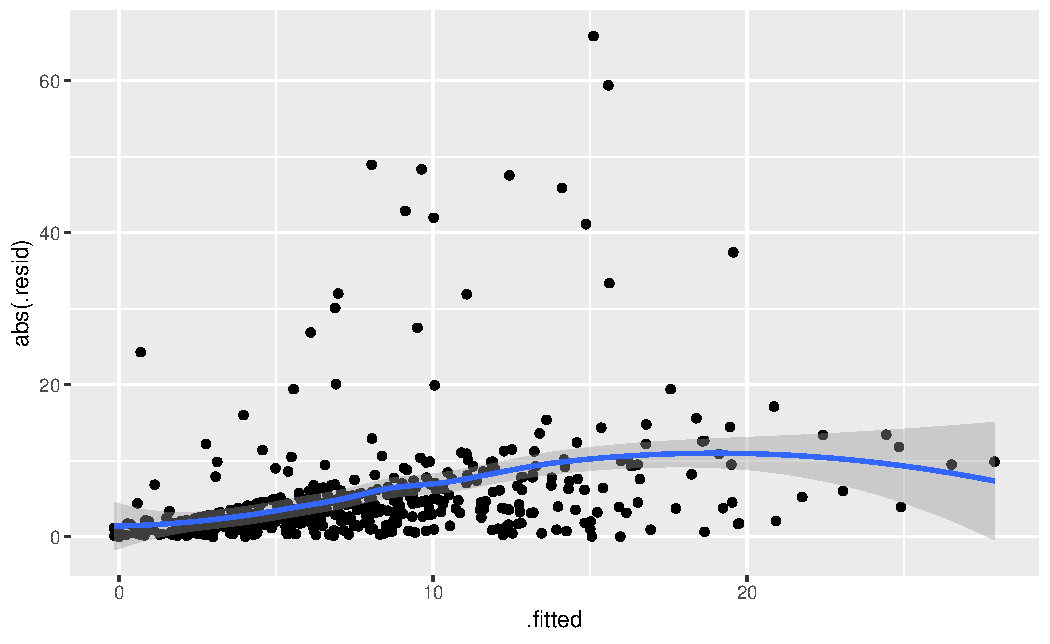
\includegraphics{figure/unnamed-chunk-36-1.pdf}
\caption{plot of chunk unnamed-chunk-36}
\end{figure}

\end{frame}

\begin{frame}{Benefit of rotation}
\protect\hypertarget{benefit-of-rotation}{}

\begin{itemize}
\item
  100m and marathon arrows almost perpendicular, but components don't
  match anything much:
\item
  sprinting: bottom left and top right
\item
  distance running: top left and bottom right.
\item
  Can we arrange things so that components (factors) correspond to
  something meaningful?
\end{itemize}

\end{frame}

\begin{frame}[fragile]{Track records by factor analysis}
\protect\hypertarget{track-records-by-factor-analysis}{}

Obtain factor scores (have actual data):

\normalsize

\begin{Shaded}
\begin{Highlighting}[]
\NormalTok{track }\OperatorTok
\StringTok{  }\KeywordTok{select_if}\NormalTok{(is.numeric) }\OperatorTok
\StringTok{  }\KeywordTok{factanal}\NormalTok{(}\DecValTok{2}\NormalTok{, }\DataTypeTok{scores =} \StringTok{"r"}\NormalTok{) ->}\StringTok{ }\NormalTok{track.f}
\end{Highlighting}
\end{Shaded}

\normalsize

\end{frame}

\begin{frame}[fragile]{Track data biplot}
\protect\hypertarget{track-data-biplot}{}

Not so nice-looking:

\begin{Shaded}
\begin{Highlighting}[]
\KeywordTok{biplot}\NormalTok{(track.f}\OperatorTok{$}\NormalTok{scores, track.f}\OperatorTok{$}\NormalTok{loadings,}
  \DataTypeTok{xlabs =}\NormalTok{ track}\OperatorTok{$}\NormalTok{country}
\NormalTok{)}
\end{Highlighting}
\end{Shaded}

\begin{figure}
\centering
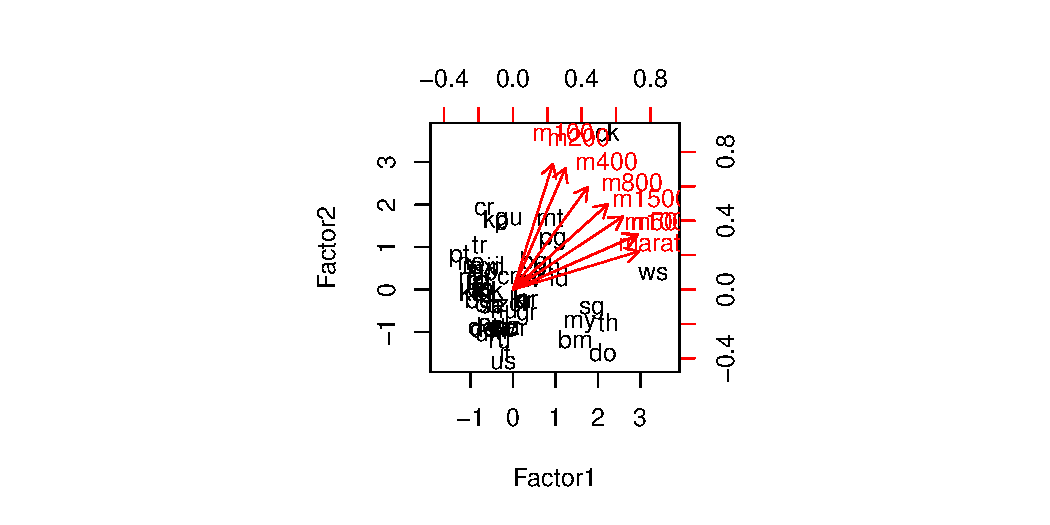
\includegraphics{figure/siracusa-1.pdf}
\caption{plot of chunk siracusa}
\end{figure}

\end{frame}

\begin{frame}{Comments}
\protect\hypertarget{comments-7}{}

\begin{itemize}
\item
  This time 100m ``up'' (factor 2), marathon ``right'' (factor 1).
\item
  Countries most negative on factor 2 good at sprinting.
\item
  Countries most negative on factor 1 good at distance running.
\end{itemize}

\end{frame}

\begin{frame}[fragile]{Rotated factor loadings}
\protect\hypertarget{rotated-factor-loadings}{}

\small

\begin{Shaded}
\begin{Highlighting}[]
\NormalTok{track.f}\OperatorTok{$}\NormalTok{loadings}
\end{Highlighting}
\end{Shaded}

\begin{verbatim}
## 
## Loadings:
##          Factor1 Factor2
## m100     0.291   0.914  
## m200     0.382   0.882  
## m400     0.543   0.744  
## m800     0.691   0.622  
## m1500    0.799   0.530  
## m5000    0.901   0.394  
## m10000   0.907   0.399  
## marathon 0.915   0.278  
## 
##                Factor1 Factor2
## SS loadings      4.112   3.225
## Proportion Var   0.514   0.403
## Cumulative Var   0.514   0.917
\end{verbatim}

\normalsize

\end{frame}

\begin{frame}[fragile]{Which countries are good at sprinting or distance
running?}
\protect\hypertarget{which-countries-are-good-at-sprinting-or-distance-running}{}

Make a data frame with the countries and scores in:

\begin{Shaded}
\begin{Highlighting}[]
\NormalTok{scores <-}\StringTok{ }\KeywordTok{data.frame}\NormalTok{(}
  \DataTypeTok{country =}\NormalTok{ track}\OperatorTok{$}\NormalTok{country,}
\NormalTok{  track.f}\OperatorTok{$}\NormalTok{scores}
\NormalTok{)}
\NormalTok{scores }\OperatorTok\StringTok{ }\KeywordTok{slice}\NormalTok{(}\DecValTok{1}\OperatorTok{:}\DecValTok{6}\NormalTok{)}
\end{Highlighting}
\end{Shaded}

\begin{verbatim}
##   country     Factor1    Factor2
## 1      ar  0.33633782 -0.2651512
## 2      au -0.49395787 -0.8121335
## 3      at -0.74199914  0.1764151
## 4      be -0.79602754 -0.2388525
## 5      bm  1.46541593 -1.1704466
## 6      br  0.07780163 -0.8871291
\end{verbatim}

\end{frame}

\begin{frame}[fragile]{The best sprinting countries}
\protect\hypertarget{the-best-sprinting-countries}{}

Most negative on factor 2:

\footnotesize

\begin{Shaded}
\begin{Highlighting}[]
\NormalTok{scores }\OperatorTok
\StringTok{  }\KeywordTok{arrange}\NormalTok{(Factor2) }\OperatorTok
\StringTok{  }\KeywordTok{left_join}\NormalTok{(iso, }\DataTypeTok{by =} \KeywordTok{c}\NormalTok{(}\StringTok{"country"}\NormalTok{ =}\StringTok{ "ISO2"}\NormalTok{)) }\OperatorTok
\StringTok{  }\KeywordTok{select}\NormalTok{(Country, Factor1, Factor2) }\OperatorTok
\StringTok{  }\KeywordTok{slice}\NormalTok{(}\DecValTok{1}\OperatorTok{:}\DecValTok{10}\NormalTok{)}
\end{Highlighting}
\end{Shaded}

\begin{verbatim}
##                     Country     Factor1    Factor2
## 1  United States of America -0.21942697 -1.7251036
## 2                     Italy -0.18436705 -1.4990521
## 3        Dominican Republic  2.12906546 -1.4666402
## 4        Russian Federation -0.32473110 -1.2236590
## 5                   Bermuda  1.46541593 -1.1704466
## 6            United Kingdom -0.58969058 -1.0139983
## 7                    France -0.25301846 -0.9519162
## 8              West Germany -0.46748876 -0.9079005
## 9                    Canada -0.13690160 -0.8920777
## 10                   Brazil  0.07780163 -0.8871291
\end{verbatim}

\normalsize

\end{frame}

\begin{frame}[fragile]{The best distance-running countries}
\protect\hypertarget{the-best-distance-running-countries}{}

Most negative on factor 1:

\footnotesize

\begin{Shaded}
\begin{Highlighting}[]
\NormalTok{scores }\OperatorTok
\StringTok{  }\KeywordTok{arrange}\NormalTok{(Factor1) }\OperatorTok
\StringTok{  }\KeywordTok{left_join}\NormalTok{(iso, }\DataTypeTok{by =} \KeywordTok{c}\NormalTok{(}\StringTok{"country"}\NormalTok{ =}\StringTok{ "ISO2"}\NormalTok{)) }\OperatorTok
\StringTok{  }\KeywordTok{select}\NormalTok{(Country, Factor1, Factor2) }\OperatorTok
\StringTok{  }\KeywordTok{slice}\NormalTok{(}\DecValTok{1}\OperatorTok{:}\DecValTok{10}\NormalTok{)}
\end{Highlighting}
\end{Shaded}

\begin{verbatim}
##                      Country    Factor1     Factor2
## 1                   Portugal -1.2509805  0.78366889
## 2                     Norway -0.9920727  0.62299560
## 3                New Zealand -0.9813348  0.26603491
## 4                      Kenya -0.9749696 -0.07099477
## 5  Iran, Islamic Republic of -0.9231505  0.50271208
## 6                Netherlands -0.9078661  0.23948200
## 7                    Romania -0.8178386  0.18555001
## 8                     Mexico -0.8096291  0.51446762
## 9                    Finland -0.8094725 -0.05705220
## 10                   Belgium -0.7960275 -0.23885253
\end{verbatim}

\normalsize

\end{frame}

\begin{frame}{A bigger example: BEM sex role inventory}
\protect\hypertarget{a-bigger-example-bem-sex-role-inventory}{}

\begin{itemize}
\item
  369 women asked to rate themselves on 60 traits, like ``self-reliant''
  or ``shy''.
\item
  Rating 1 ``never or almost never true of me'' to 7 ``always or almost
  always true of me''.
\item
  60 personality traits is a lot. Can we find a smaller number of
  factors that capture aspects of personality?
\item
  The whole BEM sex role inventory on next page.
\end{itemize}

\end{frame}

\begin{frame}{The whole inventory}
\protect\hypertarget{the-whole-inventory}{}

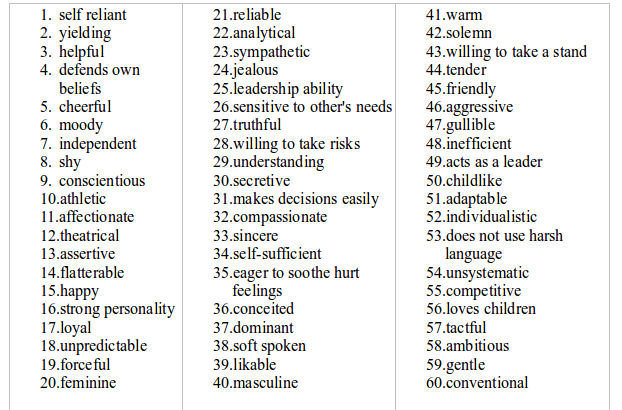
\includegraphics[width=4.6875in,height=\textheight]{bem.png}

\end{frame}

\begin{frame}[fragile]{Some of the data}
\protect\hypertarget{some-of-the-data}{}

\scriptsize

\begin{Shaded}
\begin{Highlighting}[]
\NormalTok{my_url <-}\StringTok{ "http://www.utsc.utoronto.ca/~butler/d29/factor.txt"}
\NormalTok{bem <-}\StringTok{ }\KeywordTok{read_tsv}\NormalTok{(my_url)}
\NormalTok{bem}
\end{Highlighting}
\end{Shaded}

\begin{verbatim}
## # A tibble: 369 x 45
##    subno helpful reliant defbel yielding cheerful indpt athlet
##    <dbl>   <dbl>   <dbl>  <dbl>    <dbl>    <dbl> <dbl>  <dbl>
##  1     1       7       7      5        5        7     7      7
##  2     2       5       6      6        6        2     3      3
##  3     3       7       6      4        4        5     5      2
##  4     4       6       6      7        4        6     6      3
##  5     5       6       6      7        4        7     7      7
##  6     7       5       6      7        4        6     6      2
##  7     8       6       4      6        6        6     3      1
##  8     9       7       6      7        5        6     7      5
##  9    10       7       6      6        4        4     5      2
## 10    11       7       4      7        4        7     5      2
## # … with 359 more rows, and 37 more variables: shy <dbl>,
## #   assert <dbl>, strpers <dbl>, forceful <dbl>, affect <dbl>,
## #   flatter <dbl>, loyal <dbl>, analyt <dbl>, feminine <dbl>,
## #   sympathy <dbl>, moody <dbl>, sensitiv <dbl>, undstand <dbl>,
## #   compass <dbl>, leaderab <dbl>, soothe <dbl>, risk <dbl>,
## #   decide <dbl>, selfsuff <dbl>, conscien <dbl>,
## #   dominant <dbl>, masculin <dbl>, stand <dbl>, happy <dbl>,
## #   softspok <dbl>, warm <dbl>, truthful <dbl>, tender <dbl>,
## #   gullible <dbl>, leadact <dbl>, childlik <dbl>,
## #   individ <dbl>, foullang <dbl>, lovchil <dbl>, compete <dbl>,
## #   ambitiou <dbl>, gentle <dbl>
\end{verbatim}

\normalsize

\end{frame}

\begin{frame}[fragile]{Principal components first}
\protect\hypertarget{principal-components-first}{}

\ldots to decide on number of factors:

\begin{Shaded}
\begin{Highlighting}[]
\NormalTok{bem.pc <-}\StringTok{ }\NormalTok{bem }\OperatorTok
\StringTok{  }\KeywordTok{select}\NormalTok{(}\OperatorTok{-}\NormalTok{subno) }\OperatorTok
\StringTok{  }\KeywordTok{princomp}\NormalTok{(}\DataTypeTok{cor =}\NormalTok{ T)}
\end{Highlighting}
\end{Shaded}

\end{frame}

\begin{frame}[fragile]{The scree plot}
\protect\hypertarget{the-scree-plot}{}

\begin{Shaded}
\begin{Highlighting}[]
\NormalTok{(g <-}\StringTok{ }\KeywordTok{ggscreeplot}\NormalTok{(bem.pc))}
\end{Highlighting}
\end{Shaded}

\begin{figure}
\centering
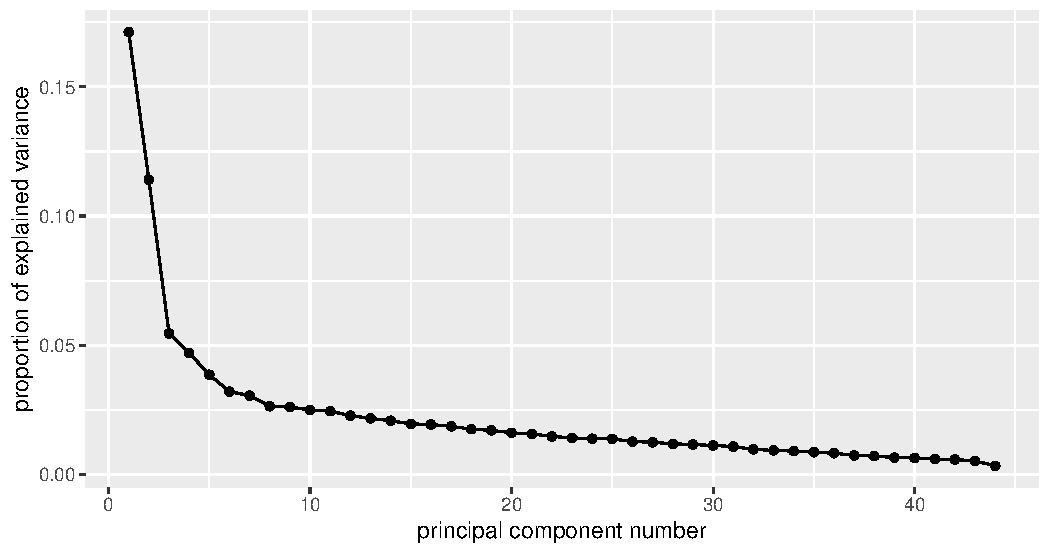
\includegraphics{figure/genoa-1.pdf}
\caption{plot of chunk genoa}
\end{figure}

\begin{itemize}
\tightlist
\item
  No obvious elbow.
\end{itemize}

\end{frame}

\begin{frame}[fragile]{Zoom in to search for elbow}
\protect\hypertarget{zoom-in-to-search-for-elbow}{}

Possible elbows at 3 (2 factors) and 6 (5):

\begin{Shaded}
\begin{Highlighting}[]
\NormalTok{g }\OperatorTok{+}\StringTok{ }\KeywordTok{scale_x_continuous}\NormalTok{(}\DataTypeTok{limits =} \KeywordTok{c}\NormalTok{(}\DecValTok{0}\NormalTok{, }\DecValTok{8}\NormalTok{))}
\end{Highlighting}
\end{Shaded}

\begin{figure}
\centering
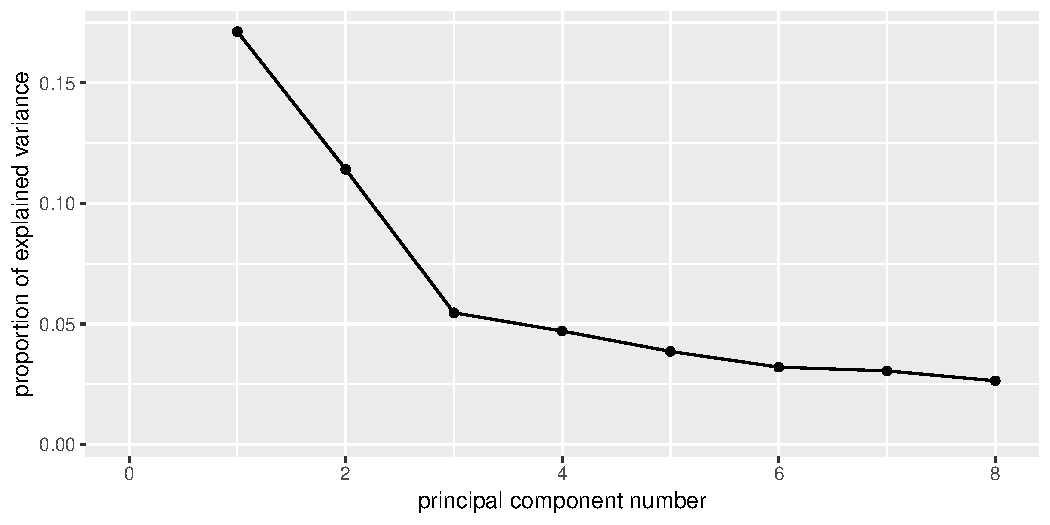
\includegraphics{figure/bem-scree-two-1.pdf}
\caption{plot of chunk bem-scree-two}
\end{figure}

\end{frame}

\begin{frame}[fragile]{but is 2 really good?}
\protect\hypertarget{but-is-2-really-good}{}

\scriptsize

\begin{Shaded}
\begin{Highlighting}[]
\KeywordTok{summary}\NormalTok{(bem.pc)}
\end{Highlighting}
\end{Shaded}

\begin{verbatim}
## Importance of components:
##                           Comp.1    Comp.2     Comp.3     Comp.4
## Standard deviation     2.7444993 2.2405789 1.55049106 1.43886350
## Proportion of Variance 0.1711881 0.1140953 0.05463688 0.04705291
## Cumulative Proportion  0.1711881 0.2852834 0.33992029 0.38697320
##                            Comp.5     Comp.6     Comp.7
## Standard deviation     1.30318840 1.18837867 1.15919129
## Proportion of Variance 0.03859773 0.03209645 0.03053919
## Cumulative Proportion  0.42557093 0.45766738 0.48820657
##                            Comp.8     Comp.9    Comp.10
## Standard deviation     1.07838912 1.07120568 1.04901318
## Proportion of Variance 0.02643007 0.02607913 0.02500974
## Cumulative Proportion  0.51463664 0.54071577 0.56572551
##                           Comp.11    Comp.12    Comp.13
## Standard deviation     1.03848656 1.00152287 0.97753974
## Proportion of Variance 0.02451033 0.02279655 0.02171782
## Cumulative Proportion  0.59023584 0.61303238 0.63475020
##                           Comp.14   Comp.15    Comp.16
## Standard deviation     0.95697572 0.9287543 0.92262649
## Proportion of Variance 0.02081369 0.0196042 0.01934636
## Cumulative Proportion  0.65556390 0.6751681 0.69451445
##                           Comp.17   Comp.18    Comp.19
## Standard deviation     0.90585705 0.8788668 0.86757525
## Proportion of Variance 0.01864948 0.0175547 0.01710652
## Cumulative Proportion  0.71316392 0.7307186 0.74782514
##                           Comp.20    Comp.21    Comp.22
## Standard deviation     0.84269120 0.83124925 0.80564654
## Proportion of Variance 0.01613928 0.01570398 0.01475151
## Cumulative Proportion  0.76396443 0.77966841 0.79441992
##                           Comp.23    Comp.24    Comp.25
## Standard deviation     0.78975423 0.78100835 0.77852606
## Proportion of Variance 0.01417527 0.01386305 0.01377506
## Cumulative Proportion  0.80859519 0.82245823 0.83623330
##                           Comp.26    Comp.27    Comp.28
## Standard deviation     0.74969868 0.74137885 0.72343693
## Proportion of Variance 0.01277382 0.01249188 0.01189457
## Cumulative Proportion  0.84900712 0.86149899 0.87339356
##                           Comp.29    Comp.30    Comp.31
## Standard deviation     0.71457305 0.70358645 0.69022738
## Proportion of Variance 0.01160488 0.01125077 0.01082759
## Cumulative Proportion  0.88499844 0.89624921 0.90707680
##                            Comp.32     Comp.33    Comp.34
## Standard deviation     0.654861232 0.640339974 0.63179848
## Proportion of Variance 0.009746437 0.009318984 0.00907203
## Cumulative Proportion  0.916823235 0.926142219 0.93521425
##                            Comp.35     Comp.36     Comp.37
## Standard deviation     0.616621295 0.602404917 0.570025368
## Proportion of Variance 0.008641405 0.008247538 0.007384748
## Cumulative Proportion  0.943855654 0.952103192 0.959487940
##                            Comp.38     Comp.39     Comp.40
## Standard deviation     0.560881809 0.538149460 0.530277613
## Proportion of Variance 0.007149736 0.006581928 0.006390781
## Cumulative Proportion  0.966637677 0.973219605 0.979610386
##                            Comp.41     Comp.42     Comp.43
## Standard deviation     0.512370708 0.505662309 0.480413465
## Proportion of Variance 0.005966449 0.005811236 0.005245389
## Cumulative Proportion  0.985576834 0.991388070 0.996633459
##                            Comp.44
## Standard deviation     0.384873772
## Proportion of Variance 0.003366541
## Cumulative Proportion  1.000000000
\end{verbatim}

\normalsize

\end{frame}

\begin{frame}{Comments}
\protect\hypertarget{comments-8}{}

\begin{itemize}
\item
  Want overall fraction of variance explained (``cumulative
  proportion'') to be reasonably high.
\item
  2 factors, 28.5\%. Terrible!
\item
  Even 56\% (10 factors) not that good!
\item
  Have to live with that.
\end{itemize}

\end{frame}

\begin{frame}[fragile]{Biplot}
\protect\hypertarget{biplot-1}{}

\begin{Shaded}
\begin{Highlighting}[]
\KeywordTok{ggbiplot}\NormalTok{(bem.pc, }\DataTypeTok{alpha =} \FloatTok{0.3}\NormalTok{)}
\end{Highlighting}
\end{Shaded}

\begin{figure}
\centering
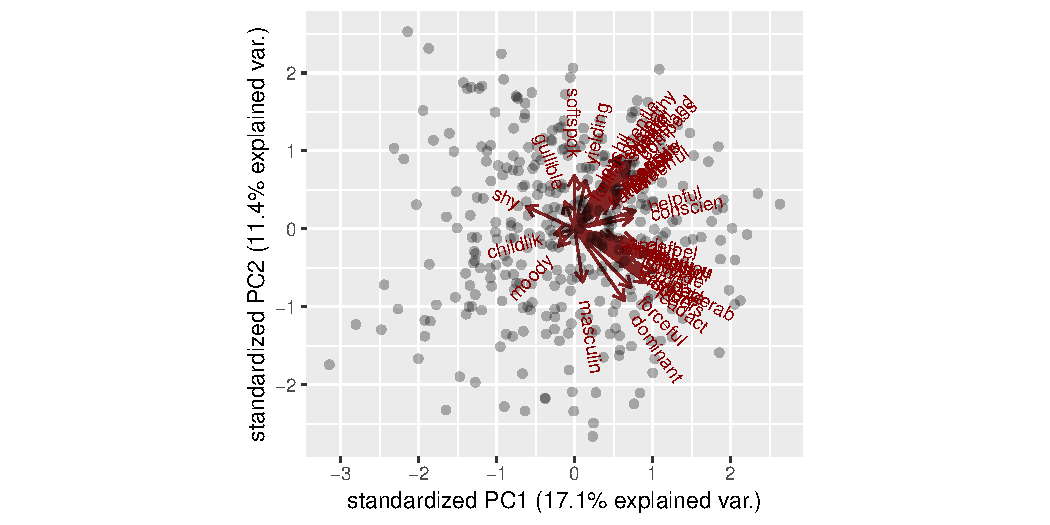
\includegraphics{figure/bem-biplot-1.pdf}
\caption{plot of chunk bem-biplot}
\end{figure}

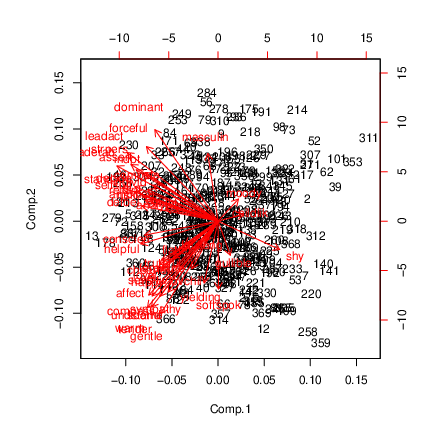
\includegraphics{bFactor-bem-biplot.png}

\end{frame}

\begin{frame}[fragile]{Comments}
\protect\hypertarget{comments-9}{}

\begin{itemize}
\item
  Ignore individuals for now.
\item
  Most variables point to 10 o'clock or 7 o'clock.
\item
  Suggests factor analysis with rotation will get interpretable factors
  (rotate to 6 o'clock and 9 o'clock, for example).
\item
  Try for 2-factor solution (rough interpretation, will be bad):
\end{itemize}

\begin{Shaded}
\begin{Highlighting}[]
\NormalTok{bem}\FloatTok{.2}\NormalTok{ <-}\StringTok{ }\NormalTok{bem }\OperatorTok
\StringTok{  }\KeywordTok{select}\NormalTok{(}\OperatorTok{-}\NormalTok{subno) }\OperatorTok
\StringTok{  }\KeywordTok{factanal}\NormalTok{(}\DataTypeTok{factors =} \DecValTok{2}\NormalTok{)}
\end{Highlighting}
\end{Shaded}

\begin{itemize}
\tightlist
\item
  Show output in pieces (just print \texttt{bem.2} to see all of it).
\end{itemize}

\end{frame}

\begin{frame}[fragile]{Uniquenesses, sorted}
\protect\hypertarget{uniquenesses-sorted}{}

\scriptsize

\begin{Shaded}
\begin{Highlighting}[]
\KeywordTok{sort}\NormalTok{(bem}\FloatTok{.2}\OperatorTok{$}\NormalTok{uniquenesses)}
\end{Highlighting}
\end{Shaded}

\begin{verbatim}
##  leaderab   leadact      warm    tender  dominant    gentle 
## 0.4091894 0.4166153 0.4764762 0.4928919 0.4942909 0.5064551 
##  forceful   strpers   compass     stand  undstand    assert 
## 0.5631857 0.5679398 0.5937073 0.6024001 0.6194392 0.6329347 
##    soothe    affect    decide  selfsuff  sympathy     indpt 
## 0.6596103 0.6616625 0.6938578 0.7210246 0.7231450 0.7282742 
##   helpful    defbel      risk   reliant   individ   compete 
## 0.7598223 0.7748448 0.7789761 0.7808058 0.7941998 0.7942910 
##  conscien     happy  sensitiv     loyal  ambitiou       shy 
## 0.7974820 0.8008966 0.8018851 0.8035264 0.8101599 0.8239496 
##  softspok  cheerful  masculin  yielding  feminine  truthful 
## 0.8339058 0.8394916 0.8453368 0.8688473 0.8829927 0.8889983 
##   lovchil    analyt    athlet   flatter  gullible     moody 
## 0.8924392 0.8968744 0.9229702 0.9409500 0.9583435 0.9730607 
##  childlik  foullang 
## 0.9800360 0.9821662
\end{verbatim}

\normalsize

\end{frame}

\begin{frame}{Comments}
\protect\hypertarget{comments-10}{}

\begin{itemize}
\item
  Mostly high or very high (bad).
\item
  Some smaller, eg.: Leadership ability (0.409), Acts like leader
  (0.417), Warm (0.476), Tender (0.493).
\item
  Smaller uniquenesses captured by one of our two factors.
\item
  Larger uniquenesses are not: need more factors to capture them.
\end{itemize}

\end{frame}

\begin{frame}[fragile]{Factor loadings, some}
\protect\hypertarget{factor-loadings-some}{}

\scriptsize

\begin{Shaded}
\begin{Highlighting}[]
\NormalTok{bem}\FloatTok{.2}\OperatorTok{$}\NormalTok{loadings}
\end{Highlighting}
\end{Shaded}

\begin{verbatim}
## 
## Loadings:
##          Factor1 Factor2
## helpful   0.314   0.376 
## reliant   0.453   0.117 
## defbel    0.434   0.193 
## yielding -0.131   0.338 
## cheerful  0.152   0.371 
## indpt     0.521         
## athlet    0.267         
## shy      -0.414         
## assert    0.605         
## strpers   0.657         
## forceful  0.649  -0.126 
## affect    0.178   0.554 
## flatter           0.223 
## loyal     0.151   0.417 
## analyt    0.295   0.127 
## feminine  0.113   0.323 
## sympathy          0.526 
## moody            -0.162 
## sensitiv  0.135   0.424 
## undstand          0.610 
## compass   0.114   0.627 
## leaderab  0.765         
## soothe            0.580 
## risk      0.442   0.161 
## decide    0.542   0.113 
## selfsuff  0.511   0.134 
## conscien  0.328   0.308 
## dominant  0.668  -0.245 
## masculin  0.276  -0.280 
## stand     0.607   0.172 
## happy     0.119   0.430 
## softspok -0.230   0.336 
## warm              0.719 
## truthful  0.109   0.315 
## tender            0.710 
## gullible -0.153   0.135 
## leadact   0.763         
## childlik -0.101         
## individ   0.445         
## foullang          0.133 
## lovchil           0.327 
## compete   0.450         
## ambitiou  0.414   0.137 
## gentle            0.702 
## 
##                Factor1 Factor2
## SS loadings      6.083   5.127
## Proportion Var   0.138   0.117
## Cumulative Var   0.138   0.255
\end{verbatim}

\normalsize

\end{frame}

\begin{frame}[fragile]{Making a data frame}
\protect\hypertarget{making-a-data-frame}{}

There are too many to read easily, so make a data frame. A bit tricky:

\footnotesize

\begin{Shaded}
\begin{Highlighting}[]
\NormalTok{loadings <-}\StringTok{ }\KeywordTok{as.data.frame}\NormalTok{(}\KeywordTok{unclass}\NormalTok{(bem}\FloatTok{.2}\OperatorTok{$}\NormalTok{loadings)) }\OperatorTok
\StringTok{  }\KeywordTok{mutate}\NormalTok{(}\DataTypeTok{trait =} \KeywordTok{rownames}\NormalTok{(bem}\FloatTok{.2}\OperatorTok{$}\NormalTok{loadings))}
\NormalTok{loadings }\OperatorTok\StringTok{ }\KeywordTok{slice}\NormalTok{(}\DecValTok{1}\OperatorTok{:}\DecValTok{12}\NormalTok{)}
\end{Highlighting}
\end{Shaded}

\begin{verbatim}
##       Factor1      Factor2    trait
## 1   0.3137466  0.376484908  helpful
## 2   0.4532904  0.117140647  reliant
## 3   0.4336574  0.192602996   defbel
## 4  -0.1309965  0.337629288 yielding
## 5   0.1523718  0.370530549 cheerful
## 6   0.5212403  0.005870336    indpt
## 7   0.2670788  0.075542858   athlet
## 8  -0.4144579 -0.065372760      shy
## 9   0.6049588  0.033004846   assert
## 10  0.6569855  0.020777649  strpers
## 11  0.6487190 -0.126405816 forceful
## 12  0.1778911  0.553799444   affect
\end{verbatim}

\normalsize

\end{frame}

\begin{frame}[fragile]{Pick out the big ones on factor 1}
\protect\hypertarget{pick-out-the-big-ones-on-factor-1}{}

Arbitrarily defining \(>0.4\) or \(<-0.4\) as ``big'':

\scriptsize

\begin{Shaded}
\begin{Highlighting}[]
\NormalTok{loadings }\OperatorTok\StringTok{ }\KeywordTok{filter}\NormalTok{(}\KeywordTok{abs}\NormalTok{(Factor1) }\OperatorTok{>}\StringTok{ }\FloatTok{0.4}\NormalTok{) }
\end{Highlighting}
\end{Shaded}

\begin{verbatim}
##       Factor1      Factor2    trait
## 1   0.4532904  0.117140647  reliant
## 2   0.4336574  0.192602996   defbel
## 3   0.5212403  0.005870336    indpt
## 4  -0.4144579 -0.065372760      shy
## 5   0.6049588  0.033004846   assert
## 6   0.6569855  0.020777649  strpers
## 7   0.6487190 -0.126405816 forceful
## 8   0.7654924  0.069513572 leaderab
## 9   0.4416176  0.161238425     risk
## 10  0.5416796  0.112807957   decide
## 11  0.5109964  0.133626767 selfsuff
## 12  0.6676490 -0.244855780 dominant
## 13  0.6066864  0.171848896    stand
## 14  0.7627129 -0.040667202  leadact
## 15  0.4448064  0.089146147  individ
## 16  0.4504188  0.053207281  compete
## 17  0.4136498  0.136869589 ambitiou
\end{verbatim}

\normalsize

\end{frame}

\begin{frame}[fragile]{Factor 2, the big ones}
\protect\hypertarget{factor-2-the-big-ones}{}

\footnotesize

\begin{Shaded}
\begin{Highlighting}[]
\NormalTok{loadings }\OperatorTok\StringTok{ }\KeywordTok{filter}\NormalTok{(}\KeywordTok{abs}\NormalTok{(Factor2) }\OperatorTok{>}\StringTok{ }\FloatTok{0.4}\NormalTok{)}
\end{Highlighting}
\end{Shaded}

\begin{verbatim}
##        Factor1   Factor2    trait
## 1   0.17789112 0.5537994   affect
## 2   0.15121266 0.4166622    loyal
## 3   0.02301456 0.5256654 sympathy
## 4   0.13476970 0.4242037 sensitiv
## 5   0.09111299 0.6101294 undstand
## 6   0.11350643 0.6272223  compass
## 7   0.06061755 0.5802714   soothe
## 8   0.11893011 0.4300698    happy
## 9   0.07956978 0.7191610     warm
## 10  0.05113807 0.7102763   tender
## 11 -0.01873224 0.7022768   gentle
\end{verbatim}

\normalsize

\end{frame}

\begin{frame}[fragile]{Plotting the two factors}
\protect\hypertarget{plotting-the-two-factors}{}

\begin{itemize}
\item
  A bi-plot, this time with the variables reduced in size. Looking for
  unusual individuals.
\item
  Have to run \texttt{factanal} again to get factor scores for plotting.
\end{itemize}

\begin{Shaded}
\begin{Highlighting}[]
\NormalTok{bem }\OperatorTok\StringTok{ }\KeywordTok{select}\NormalTok{(}\OperatorTok{-}\NormalTok{subno) }\OperatorTok\StringTok{ }
\StringTok{  }\KeywordTok{factanal}\NormalTok{(}\DataTypeTok{factors =} \DecValTok{2}\NormalTok{, }\DataTypeTok{scores =} \StringTok{"r"}\NormalTok{) ->}\StringTok{ }\NormalTok{bem}\FloatTok{.2}\NormalTok{a}
\KeywordTok{biplot}\NormalTok{(bem}\FloatTok{.2}\NormalTok{a}\OperatorTok{$}\NormalTok{scores, bem}\FloatTok{.2}\NormalTok{a}\OperatorTok{$}\NormalTok{loadings, }\DataTypeTok{cex =} \KeywordTok{c}\NormalTok{(}\FloatTok{0.5}\NormalTok{, }\FloatTok{0.5}\NormalTok{))}
\end{Highlighting}
\end{Shaded}

\begin{itemize}
\tightlist
\item
  Numbers on plot are row numbers of \texttt{bem} data frame.
\end{itemize}

\end{frame}

\begin{frame}{The (awful) biplot}
\protect\hypertarget{the-awful-biplot}{}

\begin{figure}
\centering
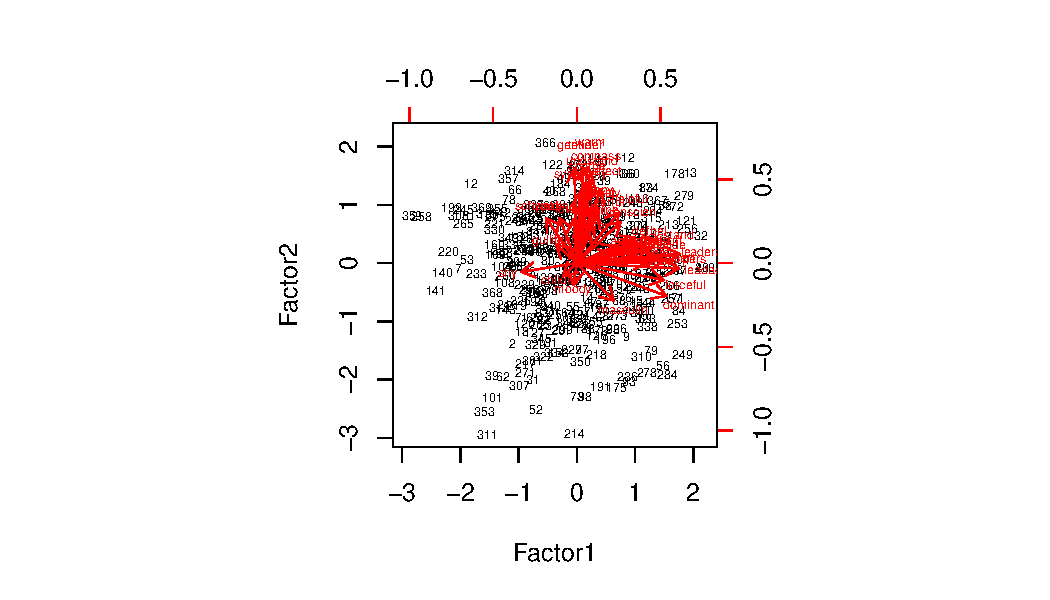
\includegraphics{figure/biplot-two-ag-1.pdf}
\caption{plot of chunk biplot-two-ag}
\end{figure}

\end{frame}

\begin{frame}{Comments}
\protect\hypertarget{comments-11}{}

\begin{itemize}
\item
  Variables mostly up (``feminine'') and right (``masculine''),
  accomplished by rotation.
\item
  Some unusual individuals: 311, 214 (low on factor 2), 366 (high on
  factor 2), 359, 258 (low on factor 1), 230 (high on factor 1).
\end{itemize}

\end{frame}

\begin{frame}[fragile]{Individual 366}
\protect\hypertarget{individual-366}{}

\tiny

\begin{Shaded}
\begin{Highlighting}[]
\NormalTok{bem }\OperatorTok\StringTok{ }\KeywordTok{slice}\NormalTok{(}\DecValTok{366}\NormalTok{) }\OperatorTok\StringTok{ }\KeywordTok{glimpse}\NormalTok{()}
\end{Highlighting}
\end{Shaded}

\begin{verbatim}
## Observations: 1
## Variables: 45
## $ subno    <dbl> 755
## $ helpful  <dbl> 7
## $ reliant  <dbl> 7
## $ defbel   <dbl> 5
## $ yielding <dbl> 7
## $ cheerful <dbl> 7
## $ indpt    <dbl> 7
## $ athlet   <dbl> 7
## $ shy      <dbl> 2
## $ assert   <dbl> 1
## $ strpers  <dbl> 3
## $ forceful <dbl> 1
## $ affect   <dbl> 7
## $ flatter  <dbl> 9
## $ loyal    <dbl> 7
## $ analyt   <dbl> 7
## $ feminine <dbl> 7
## $ sympathy <dbl> 7
## $ moody    <dbl> 1
## $ sensitiv <dbl> 7
## $ undstand <dbl> 7
## $ compass  <dbl> 6
## $ leaderab <dbl> 3
## $ soothe   <dbl> 7
## $ risk     <dbl> 7
## $ decide   <dbl> 7
## $ selfsuff <dbl> 7
## $ conscien <dbl> 7
## $ dominant <dbl> 1
## $ masculin <dbl> 1
## $ stand    <dbl> 7
## $ happy    <dbl> 7
## $ softspok <dbl> 7
## $ warm     <dbl> 7
## $ truthful <dbl> 7
## $ tender   <dbl> 7
## $ gullible <dbl> 1
## $ leadact  <dbl> 2
## $ childlik <dbl> 1
## $ individ  <dbl> 5
## $ foullang <dbl> 7
## $ lovchil  <dbl> 7
## $ compete  <dbl> 7
## $ ambitiou <dbl> 7
## $ gentle   <dbl> 7
\end{verbatim}

\normalsize

\end{frame}

\begin{frame}{Comments}
\protect\hypertarget{comments-12}{}

\begin{itemize}
\item
  Individual 366 high on factor 2, but hard to see which traits should
  have high scores (unless we remember).
\item
  Idea: \emph{tidy} original data frame to make easier to look things
  up.
\end{itemize}

\end{frame}

\begin{frame}[fragile]{Tidying original data}
\protect\hypertarget{tidying-original-data}{}

\scriptsize

\begin{Shaded}
\begin{Highlighting}[]
\NormalTok{bem_tidy <-}\StringTok{ }\NormalTok{bem }\OperatorTok
\StringTok{  }\KeywordTok{mutate}\NormalTok{(}\DataTypeTok{row =} \KeywordTok{row_number}\NormalTok{()) }\OperatorTok
\StringTok{  }\KeywordTok{gather}\NormalTok{(trait, score, }\KeywordTok{c}\NormalTok{(}\OperatorTok{-}\NormalTok{subno, }\OperatorTok{-}\NormalTok{row))}
\NormalTok{bem_tidy}
\end{Highlighting}
\end{Shaded}

\begin{verbatim}
## # A tibble: 16,236 x 4
##    subno   row trait   score
##    <dbl> <int> <chr>   <dbl>
##  1     1     1 helpful     7
##  2     2     2 helpful     5
##  3     3     3 helpful     7
##  4     4     4 helpful     6
##  5     5     5 helpful     6
##  6     7     6 helpful     5
##  7     8     7 helpful     6
##  8     9     8 helpful     7
##  9    10     9 helpful     7
## 10    11    10 helpful     7
## # … with 16,226 more rows
\end{verbatim}

\normalsize

\end{frame}

\begin{frame}[fragile]{Recall data frame of loadings}
\protect\hypertarget{recall-data-frame-of-loadings}{}

\footnotesize

\begin{Shaded}
\begin{Highlighting}[]
\NormalTok{loadings }\OperatorTok\StringTok{ }\KeywordTok{slice}\NormalTok{(}\DecValTok{1}\OperatorTok{:}\DecValTok{10}\NormalTok{)}
\end{Highlighting}
\end{Shaded}

\begin{verbatim}
##       Factor1      Factor2    trait
## 1   0.3137466  0.376484908  helpful
## 2   0.4532904  0.117140647  reliant
## 3   0.4336574  0.192602996   defbel
## 4  -0.1309965  0.337629288 yielding
## 5   0.1523718  0.370530549 cheerful
## 6   0.5212403  0.005870336    indpt
## 7   0.2670788  0.075542858   athlet
## 8  -0.4144579 -0.065372760      shy
## 9   0.6049588  0.033004846   assert
## 10  0.6569855  0.020777649  strpers
\end{verbatim}

\normalsize

Want to add the factor scores for each trait to our tidy data frame
\texttt{bem\_tidy}. This is a left-join (over), matching on the column
\texttt{trait} that is in both data frames (thus, the default):

\end{frame}

\begin{frame}[fragile]{Looking up loadings}
\protect\hypertarget{looking-up-loadings}{}

\scriptsize

\begin{Shaded}
\begin{Highlighting}[]
\NormalTok{bem_tidy }\OperatorTok\StringTok{ }\KeywordTok{left_join}\NormalTok{(loadings) ->}\StringTok{ }\NormalTok{bem_tidy}
\end{Highlighting}
\end{Shaded}

\begin{verbatim}
## Joining, by = "trait"
\end{verbatim}

\begin{Shaded}
\begin{Highlighting}[]
\NormalTok{bem_tidy }\OperatorTok\StringTok{ }\KeywordTok{sample_n}\NormalTok{(}\DecValTok{12}\NormalTok{)}
\end{Highlighting}
\end{Shaded}

\begin{verbatim}
## # A tibble: 12 x 6
##    subno   row trait    score Factor1 Factor2
##    <dbl> <int> <chr>    <dbl>   <dbl>   <dbl>
##  1    98    60 decide       4  0.542   0.113 
##  2   247   141 compete      4  0.450   0.0532
##  3   104    64 decide       5  0.542   0.113 
##  4   365   213 affect       7  0.178   0.554 
##  5   266   154 shy          1 -0.414  -0.0654
##  6   528   307 helpful      6  0.314   0.376 
##  7   214   123 decide       6  0.542   0.113 
##  8   245   139 compass      7  0.114   0.627 
##  9   146    95 yielding     3 -0.131   0.338 
## 10   689   354 tender       6  0.0511  0.710 
## 11   467   265 forceful     1  0.649  -0.126 
## 12   461   260 truthful     6  0.109   0.315
\end{verbatim}

\normalsize

\end{frame}

\begin{frame}[fragile]{Individual 366, high on Factor 2}
\protect\hypertarget{individual-366-high-on-factor-2}{}

So now pick out the rows of the tidy data frame that belong to
individual 366 (\texttt{row=366}) and for which the \texttt{Factor2}
score exceeds 0.4 in absolute value (our ``big'' from before):

\scriptsize

\begin{Shaded}
\begin{Highlighting}[]
\NormalTok{bem_tidy }\OperatorTok\StringTok{ }\KeywordTok{filter}\NormalTok{(row }\OperatorTok{==}\StringTok{ }\DecValTok{366}\NormalTok{, }\KeywordTok{abs}\NormalTok{(Factor2) }\OperatorTok{>}\StringTok{ }\FloatTok{0.4}\NormalTok{)}
\end{Highlighting}
\end{Shaded}

\begin{verbatim}
## # A tibble: 11 x 6
##    subno   row trait    score Factor1 Factor2
##    <dbl> <int> <chr>    <dbl>   <dbl>   <dbl>
##  1   755   366 affect       7  0.178    0.554
##  2   755   366 loyal        7  0.151    0.417
##  3   755   366 sympathy     7  0.0230   0.526
##  4   755   366 sensitiv     7  0.135    0.424
##  5   755   366 undstand     7  0.0911   0.610
##  6   755   366 compass      6  0.114    0.627
##  7   755   366 soothe       7  0.0606   0.580
##  8   755   366 happy        7  0.119    0.430
##  9   755   366 warm         7  0.0796   0.719
## 10   755   366 tender       7  0.0511   0.710
## 11   755   366 gentle       7 -0.0187   0.702
\end{verbatim}

\normalsize

As expected, high scorer on these.

\end{frame}

\begin{frame}[fragile]{Several individuals}
\protect\hypertarget{several-individuals}{}

Rows 311 and 214 were \emph{low} on Factor 2, so their scores should be
low. Can we do them all at once?

\footnotesize

\begin{Shaded}
\begin{Highlighting}[]
\NormalTok{bem_tidy }\OperatorTok\StringTok{ }\KeywordTok{filter}\NormalTok{(}
\NormalTok{  row }\OperatorTok\StringTok{ }\KeywordTok{c}\NormalTok{(}\DecValTok{366}\NormalTok{, }\DecValTok{311}\NormalTok{, }\DecValTok{214}\NormalTok{),}
  \KeywordTok{abs}\NormalTok{(Factor2) }\OperatorTok{>}\StringTok{ }\FloatTok{0.4}
\NormalTok{)}
\end{Highlighting}
\end{Shaded}

\begin{verbatim}
## # A tibble: 33 x 6
##    subno   row trait    score Factor1 Factor2
##    <dbl> <int> <chr>    <dbl>   <dbl>   <dbl>
##  1   369   214 affect       1  0.178    0.554
##  2   534   311 affect       5  0.178    0.554
##  3   755   366 affect       7  0.178    0.554
##  4   369   214 loyal        7  0.151    0.417
##  5   534   311 loyal        4  0.151    0.417
##  6   755   366 loyal        7  0.151    0.417
##  7   369   214 sympathy     4  0.0230   0.526
##  8   534   311 sympathy     4  0.0230   0.526
##  9   755   366 sympathy     7  0.0230   0.526
## 10   369   214 sensitiv     7  0.135    0.424
## # … with 23 more rows
\end{verbatim}

\normalsize

Can we display each individual in own column?

\end{frame}

\begin{frame}[fragile]{Individual by column}
\protect\hypertarget{individual-by-column}{}

Un-\texttt{tidy}, that is, \texttt{spread}:

\tiny

\begin{Shaded}
\begin{Highlighting}[]
\NormalTok{bem_tidy }\OperatorTok
\StringTok{  }\KeywordTok{filter}\NormalTok{(}
\NormalTok{    row }\OperatorTok\StringTok{ }\KeywordTok{c}\NormalTok{(}\DecValTok{366}\NormalTok{, }\DecValTok{311}\NormalTok{, }\DecValTok{214}\NormalTok{),}
    \KeywordTok{abs}\NormalTok{(Factor2) }\OperatorTok{>}\StringTok{ }\FloatTok{0.4}
\NormalTok{  ) }\OperatorTok
\StringTok{  }\KeywordTok{select}\NormalTok{(}\OperatorTok{-}\NormalTok{subno, }\OperatorTok{-}\NormalTok{Factor1, }\OperatorTok{-}\NormalTok{Factor2) }\OperatorTok
\StringTok{  }\KeywordTok{spread}\NormalTok{(row, score)}
\end{Highlighting}
\end{Shaded}

\begin{verbatim}
## # A tibble: 11 x 4
##    trait    `214` `311` `366`
##    <chr>    <dbl> <dbl> <dbl>
##  1 affect       1     5     7
##  2 compass      5     4     6
##  3 gentle       2     3     7
##  4 happy        4     3     7
##  5 loyal        7     4     7
##  6 sensitiv     7     4     7
##  7 soothe       3     4     7
##  8 sympathy     4     4     7
##  9 tender       3     4     7
## 10 undstand     5     3     7
## 11 warm         1     3     7
\end{verbatim}

\normalsize

366 high, 311 middling, 214 (sometimes) low.

\end{frame}

\begin{frame}[fragile]{Individuals 230, 258, 359}
\protect\hypertarget{individuals-230-258-359}{}

These were high, low, low on factor 1. Adapt code:

\tiny

\begin{Shaded}
\begin{Highlighting}[]
\NormalTok{bem_tidy }\OperatorTok
\StringTok{  }\KeywordTok{filter}\NormalTok{(row }\OperatorTok\StringTok{ }\KeywordTok{c}\NormalTok{(}\DecValTok{359}\NormalTok{, }\DecValTok{258}\NormalTok{, }\DecValTok{230}\NormalTok{), }\KeywordTok{abs}\NormalTok{(Factor1) }\OperatorTok{>}\StringTok{ }\FloatTok{0.4}\NormalTok{) }\OperatorTok
\StringTok{  }\KeywordTok{select}\NormalTok{(}\OperatorTok{-}\NormalTok{subno, }\OperatorTok{-}\NormalTok{Factor1, }\OperatorTok{-}\NormalTok{Factor2) }\OperatorTok
\StringTok{  }\KeywordTok{spread}\NormalTok{(row, score)}
\end{Highlighting}
\end{Shaded}

\begin{verbatim}
## # A tibble: 17 x 4
##    trait    `230` `258` `359`
##    <chr>    <dbl> <dbl> <dbl>
##  1 ambitiou     7     2     4
##  2 assert       7     3     1
##  3 compete      6     2     1
##  4 decide       7     1     2
##  5 defbel       7     1     1
##  6 dominant     7     1     1
##  7 forceful     7     1     1
##  8 individ      7     3     3
##  9 indpt        7     7     1
## 10 leadact      7     1     1
## 11 leaderab     7     1     1
## 12 reliant      7     4     1
## 13 risk         7     5     7
## 14 selfsuff     7     4     1
## 15 shy          2     7     5
## 16 stand        7     1     6
## 17 strpers      7     1     3
\end{verbatim}

\normalsize

\end{frame}

\begin{frame}[fragile]{Is 2 factors enough?}
\protect\hypertarget{is-2-factors-enough}{}

Suspect not:

\begin{Shaded}
\begin{Highlighting}[]
\NormalTok{bem}\FloatTok{.2}\OperatorTok{$}\NormalTok{PVAL}
\end{Highlighting}
\end{Shaded}

\begin{verbatim}
##     objective 
## 1.458183e-150
\end{verbatim}

2 factors resoundingly rejected. Need more. Have to go all the way to 15
factors to not reject:

\begin{Shaded}
\begin{Highlighting}[]
\NormalTok{bem}\FloatTok{.15}\NormalTok{ <-}\StringTok{ }\NormalTok{bem }\OperatorTok
\StringTok{  }\KeywordTok{select}\NormalTok{(}\OperatorTok{-}\NormalTok{subno) }\OperatorTok
\StringTok{  }\KeywordTok{factanal}\NormalTok{(}\DataTypeTok{factors =} \DecValTok{15}\NormalTok{)}
\NormalTok{bem}\FloatTok{.15}\OperatorTok{$}\NormalTok{PVAL}
\end{Highlighting}
\end{Shaded}

\begin{verbatim}
## objective 
##  0.132617
\end{verbatim}

Even then, only just over 50\% of variability explained.

Let's have a look at the important things in those 15 factors.

\end{frame}

\begin{frame}[fragile]{Get 15-factor loadings}
\protect\hypertarget{get-15-factor-loadings}{}

into a data frame, as before:

\small

\begin{Shaded}
\begin{Highlighting}[]
\NormalTok{loadings <-}\StringTok{ }\KeywordTok{as.data.frame}\NormalTok{(}\KeywordTok{unclass}\NormalTok{(bem}\FloatTok{.15}\OperatorTok{$}\NormalTok{loadings)) }\OperatorTok
\StringTok{  }\KeywordTok{mutate}\NormalTok{(}\DataTypeTok{trait =} \KeywordTok{rownames}\NormalTok{(bem}\FloatTok{.15}\OperatorTok{$}\NormalTok{loadings))}
\end{Highlighting}
\end{Shaded}

\normalsize

then show the highest few loadings on each factor.

\end{frame}

\begin{frame}[fragile]{Factor 1 (of 15)}
\protect\hypertarget{factor-1-of-15}{}

\footnotesize

\begin{Shaded}
\begin{Highlighting}[]
\NormalTok{loadings }\OperatorTok
\StringTok{  }\KeywordTok{arrange}\NormalTok{(}\KeywordTok{desc}\NormalTok{(}\KeywordTok{abs}\NormalTok{(Factor1))) }\OperatorTok
\StringTok{  }\KeywordTok{select}\NormalTok{(Factor1, trait) }\OperatorTok
\StringTok{  }\KeywordTok{slice}\NormalTok{(}\DecValTok{1}\OperatorTok{:}\DecValTok{10}\NormalTok{)}
\end{Highlighting}
\end{Shaded}

\begin{verbatim}
##      Factor1    trait
## 1  0.8127595  compass
## 2  0.6756043 undstand
## 3  0.6611293 sympathy
## 4  0.6408327 sensitiv
## 5  0.5971006   soothe
## 6  0.3481290     warm
## 7  0.2797159   gentle
## 8  0.2788627   tender
## 9  0.2501505  helpful
## 10 0.2340594 conscien
\end{verbatim}

\normalsize

Compassionate, understanding, sympathetic, soothing: thoughtful of
others.

\end{frame}

\begin{frame}[fragile]{Factor 2}
\protect\hypertarget{factor-2}{}

\footnotesize

\begin{Shaded}
\begin{Highlighting}[]
\NormalTok{loadings }\OperatorTok
\StringTok{  }\KeywordTok{arrange}\NormalTok{(}\KeywordTok{desc}\NormalTok{(}\KeywordTok{abs}\NormalTok{(Factor2))) }\OperatorTok
\StringTok{  }\KeywordTok{select}\NormalTok{(Factor2, trait) }\OperatorTok
\StringTok{  }\KeywordTok{slice}\NormalTok{(}\DecValTok{1}\OperatorTok{:}\DecValTok{10}\NormalTok{)}
\end{Highlighting}
\end{Shaded}

\begin{verbatim}
##       Factor2    trait
## 1   0.7615492  strpers
## 2   0.7160312 forceful
## 3   0.6981500   assert
## 4   0.5041921 dominant
## 5   0.3929344 leaderab
## 6   0.3669560    stand
## 7   0.3507080  leadact
## 8  -0.3131682 softspok
## 9  -0.2866862      shy
## 10  0.2602525   analyt
\end{verbatim}

\normalsize

Strong personality, forceful, assertive, dominant: getting ahead.

\end{frame}

\begin{frame}[fragile]{Factor 3}
\protect\hypertarget{factor-3}{}

\footnotesize

\begin{Shaded}
\begin{Highlighting}[]
\NormalTok{loadings }\OperatorTok
\StringTok{  }\KeywordTok{arrange}\NormalTok{(}\KeywordTok{desc}\NormalTok{(}\KeywordTok{abs}\NormalTok{(Factor3))) }\OperatorTok
\StringTok{  }\KeywordTok{select}\NormalTok{(Factor3, trait) }\OperatorTok
\StringTok{  }\KeywordTok{slice}\NormalTok{(}\DecValTok{1}\OperatorTok{:}\DecValTok{10}\NormalTok{)}
\end{Highlighting}
\end{Shaded}

\begin{verbatim}
##       Factor3    trait
## 1   0.6697542  reliant
## 2   0.6475496 selfsuff
## 3   0.6204018    indpt
## 4   0.3899607  helpful
## 5  -0.3393605 gullible
## 6   0.3333813  individ
## 7   0.3319003   decide
## 8   0.3294806 conscien
## 9   0.2877396 leaderab
## 10  0.2804170   defbel
\end{verbatim}

\normalsize

Self-reliant, self-sufficient, independent: going it alone.

\end{frame}

\begin{frame}[fragile]{Factor 4}
\protect\hypertarget{factor-4}{}

\footnotesize

\begin{Shaded}
\begin{Highlighting}[]
\NormalTok{loadings }\OperatorTok
\StringTok{  }\KeywordTok{arrange}\NormalTok{(}\KeywordTok{desc}\NormalTok{(}\KeywordTok{abs}\NormalTok{(Factor4))) }\OperatorTok
\StringTok{  }\KeywordTok{select}\NormalTok{(Factor4, trait) }\OperatorTok
\StringTok{  }\KeywordTok{slice}\NormalTok{(}\DecValTok{1}\OperatorTok{:}\DecValTok{10}\NormalTok{)}
\end{Highlighting}
\end{Shaded}

\begin{verbatim}
##      Factor4    trait
## 1  0.6956206   gentle
## 2  0.6920303   tender
## 3  0.5992467     warm
## 4  0.4465546   affect
## 5  0.3942568 softspok
## 6  0.2779793  lovchil
## 7  0.2444249 undstand
## 8  0.2442119    happy
## 9  0.2125905    loyal
## 10 0.2022861   soothe
\end{verbatim}

\normalsize

Gentle, tender, warm (affectionate): caring for others.

\end{frame}

\begin{frame}[fragile]{Factor 5}
\protect\hypertarget{factor-5}{}

\footnotesize

\begin{Shaded}
\begin{Highlighting}[]
\NormalTok{loadings }\OperatorTok
\StringTok{  }\KeywordTok{arrange}\NormalTok{(}\KeywordTok{desc}\NormalTok{(}\KeywordTok{abs}\NormalTok{(Factor5))) }\OperatorTok
\StringTok{  }\KeywordTok{select}\NormalTok{(Factor5, trait) }\OperatorTok
\StringTok{  }\KeywordTok{slice}\NormalTok{(}\DecValTok{1}\OperatorTok{:}\DecValTok{10}\NormalTok{)}
\end{Highlighting}
\end{Shaded}

\begin{verbatim}
##      Factor5    trait
## 1  0.6956846  compete
## 2  0.6743459 ambitiou
## 3  0.3453425     risk
## 4  0.3423456  individ
## 5  0.2808623   athlet
## 6  0.2695570 leaderab
## 7  0.2449656   decide
## 8  0.2064415 dominant
## 9  0.1928159  leadact
## 10 0.1854989  strpers
\end{verbatim}

\normalsize

Ambitious, competitive (with a bit of risk-taking and individualism):
Being the best.

\end{frame}

\begin{frame}[fragile]{Factor 6}
\protect\hypertarget{factor-6}{}

\footnotesize

\begin{Shaded}
\begin{Highlighting}[]
\NormalTok{loadings }\OperatorTok
\StringTok{  }\KeywordTok{arrange}\NormalTok{(}\KeywordTok{desc}\NormalTok{(}\KeywordTok{abs}\NormalTok{(Factor6))) }\OperatorTok
\StringTok{  }\KeywordTok{select}\NormalTok{(Factor6, trait) }\OperatorTok
\StringTok{  }\KeywordTok{slice}\NormalTok{(}\DecValTok{1}\OperatorTok{:}\DecValTok{10}\NormalTok{)}
\end{Highlighting}
\end{Shaded}

\begin{verbatim}
##       Factor6    trait
## 1   0.8675651  leadact
## 2   0.6078869 leaderab
## 3   0.3378645 dominant
## 4   0.2014835 forceful
## 5  -0.1915632      shy
## 6   0.1789256     risk
## 7   0.1703440 masculin
## 8   0.1639190   decide
## 9   0.1594585  compete
## 10  0.1466037   athlet
\end{verbatim}

\normalsize

Acts like a leader, leadership ability (with a bit of Dominant): Taking
charge.

\end{frame}

\begin{frame}[fragile]{Factor 7}
\protect\hypertarget{factor-7}{}

\footnotesize

\begin{Shaded}
\begin{Highlighting}[]
\NormalTok{loadings }\OperatorTok
\StringTok{  }\KeywordTok{arrange}\NormalTok{(}\KeywordTok{desc}\NormalTok{(}\KeywordTok{abs}\NormalTok{(Factor7))) }\OperatorTok
\StringTok{  }\KeywordTok{select}\NormalTok{(Factor7, trait) }\OperatorTok
\StringTok{  }\KeywordTok{slice}\NormalTok{(}\DecValTok{1}\OperatorTok{:}\DecValTok{10}\NormalTok{)}
\end{Highlighting}
\end{Shaded}

\begin{verbatim}
##       Factor7    trait
## 1   0.6698996    happy
## 2   0.6667105 cheerful
## 3  -0.5219125    moody
## 4   0.2191425   athlet
## 5   0.2126626     warm
## 6   0.1719953   gentle
## 7  -0.1640302 masculin
## 8   0.1601472  reliant
## 9   0.1472926 yielding
## 10  0.1410481  lovchil
\end{verbatim}

\normalsize

Acts like a leader, leadership ability (with a bit of Dominant): Taking
charge.

\end{frame}

\begin{frame}[fragile]{Factor 8}
\protect\hypertarget{factor-8}{}

\footnotesize

\begin{Shaded}
\begin{Highlighting}[]
\NormalTok{loadings }\OperatorTok
\StringTok{  }\KeywordTok{arrange}\NormalTok{(}\KeywordTok{desc}\NormalTok{(}\KeywordTok{abs}\NormalTok{(Factor8))) }\OperatorTok
\StringTok{  }\KeywordTok{select}\NormalTok{(Factor8, trait) }\OperatorTok
\StringTok{  }\KeywordTok{slice}\NormalTok{(}\DecValTok{1}\OperatorTok{:}\DecValTok{10}\NormalTok{)}
\end{Highlighting}
\end{Shaded}

\begin{verbatim}
##       Factor8    trait
## 1   0.6296764   affect
## 2   0.5158355  flatter
## 3  -0.2512066 softspok
## 4   0.2214623     warm
## 5   0.1878549   tender
## 6   0.1846225  strpers
## 7  -0.1804838      shy
## 8   0.1801992  compete
## 9   0.1658105    loyal
## 10  0.1548617  helpful
\end{verbatim}

\normalsize

Affectionate, flattering: Making others feel good.

\end{frame}

\begin{frame}[fragile]{Factor 9}
\protect\hypertarget{factor-9}{}

\footnotesize

\begin{Shaded}
\begin{Highlighting}[]
\NormalTok{loadings }\OperatorTok
\StringTok{  }\KeywordTok{arrange}\NormalTok{(}\KeywordTok{desc}\NormalTok{(}\KeywordTok{abs}\NormalTok{(Factor9))) }\OperatorTok
\StringTok{  }\KeywordTok{select}\NormalTok{(Factor9, trait) }\OperatorTok
\StringTok{  }\KeywordTok{slice}\NormalTok{(}\DecValTok{1}\OperatorTok{:}\DecValTok{10}\NormalTok{)}
\end{Highlighting}
\end{Shaded}

\begin{verbatim}
##       Factor9    trait
## 1   0.8633171    stand
## 2   0.3403294   defbel
## 3   0.2446971  individ
## 4   0.1941110     risk
## 5  -0.1715481      shy
## 6   0.1710978   decide
## 7   0.1197126   assert
## 8   0.1157729 conscien
## 9   0.1120308   analyt
## 10 -0.1115140 gullible
\end{verbatim}

\normalsize

Taking a stand.

\end{frame}

\begin{frame}[fragile]{Factor 10}
\protect\hypertarget{factor-10}{}

\footnotesize

\begin{Shaded}
\begin{Highlighting}[]
\NormalTok{loadings }\OperatorTok
\StringTok{  }\KeywordTok{arrange}\NormalTok{(}\KeywordTok{desc}\NormalTok{(}\KeywordTok{abs}\NormalTok{(Factor10))) }\OperatorTok
\StringTok{  }\KeywordTok{select}\NormalTok{(Factor10, trait) }\OperatorTok
\StringTok{  }\KeywordTok{slice}\NormalTok{(}\DecValTok{1}\OperatorTok{:}\DecValTok{10}\NormalTok{)}
\end{Highlighting}
\end{Shaded}

\begin{verbatim}
##       Factor10    trait
## 1   0.80751267 feminine
## 2  -0.26378513 masculin
## 3   0.24507184 softspok
## 4   0.23175597 conscien
## 5   0.20192035 selfsuff
## 6   0.17584233 yielding
## 7   0.14127067   gentle
## 8   0.11282028  flatter
## 9   0.10934531   decide
## 10 -0.09407978  lovchil
\end{verbatim}

\normalsize

Feminine. (A little bit of not-masculine!)

\end{frame}

\begin{frame}[fragile]{Factor 11}
\protect\hypertarget{factor-11}{}

\footnotesize

\begin{Shaded}
\begin{Highlighting}[]
\NormalTok{loadings }\OperatorTok
\StringTok{  }\KeywordTok{arrange}\NormalTok{(}\KeywordTok{desc}\NormalTok{(}\KeywordTok{abs}\NormalTok{(Factor11))) }\OperatorTok
\StringTok{  }\KeywordTok{select}\NormalTok{(Factor11, trait) }\OperatorTok
\StringTok{  }\KeywordTok{slice}\NormalTok{(}\DecValTok{1}\OperatorTok{:}\DecValTok{10}\NormalTok{)}
\end{Highlighting}
\end{Shaded}

\begin{verbatim}
##      Factor11    trait
## 1  0.91622589    loyal
## 2  0.18949077   affect
## 3  0.15883857 truthful
## 4  0.12464529  helpful
## 5  0.10440664   analyt
## 6  0.10076794   tender
## 7  0.09720457  lovchil
## 8  0.09635223 gullible
## 9  0.09350623 cheerful
## 10 0.08207596 conscien
\end{verbatim}

\normalsize

Loyal.

\end{frame}

\begin{frame}[fragile]{Factor 12}
\protect\hypertarget{factor-12}{}

\footnotesize

\begin{Shaded}
\begin{Highlighting}[]
\NormalTok{loadings }\OperatorTok
\StringTok{  }\KeywordTok{arrange}\NormalTok{(}\KeywordTok{desc}\NormalTok{(}\KeywordTok{abs}\NormalTok{(Factor12))) }\OperatorTok
\StringTok{  }\KeywordTok{select}\NormalTok{(Factor12, trait) }\OperatorTok
\StringTok{  }\KeywordTok{slice}\NormalTok{(}\DecValTok{1}\OperatorTok{:}\DecValTok{10}\NormalTok{)}
\end{Highlighting}
\end{Shaded}

\begin{verbatim}
##      Factor12    trait
## 1   0.6106933 childlik
## 2  -0.2845004 selfsuff
## 3  -0.2786751 conscien
## 4   0.2588843    moody
## 5   0.2013245      shy
## 6  -0.1669301   decide
## 7   0.1542031 masculin
## 8   0.1455526 dominant
## 9   0.1379163  compass
## 10 -0.1297408 leaderab
\end{verbatim}

\normalsize

Childlike. (With a bit of moody, shy, not-self-sufficient,
not-conscientious.)

\end{frame}

\begin{frame}[fragile]{Factor 13}
\protect\hypertarget{factor-13}{}

\footnotesize

\begin{Shaded}
\begin{Highlighting}[]
\NormalTok{loadings }\OperatorTok
\StringTok{  }\KeywordTok{arrange}\NormalTok{(}\KeywordTok{desc}\NormalTok{(}\KeywordTok{abs}\NormalTok{(Factor13))) }\OperatorTok
\StringTok{  }\KeywordTok{select}\NormalTok{(Factor13, trait) }\OperatorTok
\StringTok{  }\KeywordTok{slice}\NormalTok{(}\DecValTok{1}\OperatorTok{:}\DecValTok{10}\NormalTok{)}
\end{Highlighting}
\end{Shaded}

\begin{verbatim}
##      Factor13    trait
## 1   0.5729242 truthful
## 2  -0.2776490 gullible
## 3   0.2631046    happy
## 4   0.1885152     warm
## 5  -0.1671924      shy
## 6   0.1646031    loyal
## 7  -0.1438127 yielding
## 8  -0.1302900   assert
## 9   0.1137074   defbel
## 10 -0.1105583  lovchil
\end{verbatim}

\normalsize

Truthful. (With a bit of happy and not-gullible.)

\end{frame}

\begin{frame}[fragile]{Factor 14}
\protect\hypertarget{factor-14}{}

\footnotesize

\begin{Shaded}
\begin{Highlighting}[]
\NormalTok{loadings }\OperatorTok
\StringTok{  }\KeywordTok{arrange}\NormalTok{(}\KeywordTok{desc}\NormalTok{(}\KeywordTok{abs}\NormalTok{(Factor14))) }\OperatorTok
\StringTok{  }\KeywordTok{select}\NormalTok{(Factor14, trait) }\OperatorTok
\StringTok{  }\KeywordTok{slice}\NormalTok{(}\DecValTok{1}\OperatorTok{:}\DecValTok{10}\NormalTok{)}
\end{Highlighting}
\end{Shaded}

\begin{verbatim}
##      Factor14    trait
## 1   0.4429926   decide
## 2   0.2369714 selfsuff
## 3   0.1945034 forceful
## 4  -0.1862756 softspok
## 5   0.1604175     risk
## 6  -0.1484606  strpers
## 7   0.1461972 dominant
## 8   0.1279456    happy
## 9   0.1154479  compass
## 10  0.1054078 masculin
\end{verbatim}

\normalsize

Decisive. (With a bit of self-sufficient and not-soft-spoken.)

\end{frame}

\begin{frame}[fragile]{Factor 15}
\protect\hypertarget{factor-15}{}

\footnotesize

\begin{Shaded}
\begin{Highlighting}[]
\NormalTok{loadings }\OperatorTok
\StringTok{  }\KeywordTok{arrange}\NormalTok{(}\KeywordTok{desc}\NormalTok{(}\KeywordTok{abs}\NormalTok{(Factor15))) }\OperatorTok
\StringTok{  }\KeywordTok{select}\NormalTok{(Factor15, trait) }\OperatorTok
\StringTok{  }\KeywordTok{slice}\NormalTok{(}\DecValTok{1}\OperatorTok{:}\DecValTok{10}\NormalTok{)}
\end{Highlighting}
\end{Shaded}

\begin{verbatim}
##      Factor15    trait
## 1  -0.3244092  compass
## 2   0.2471884   athlet
## 3   0.2292980 sensitiv
## 4   0.1986878     risk
## 5  -0.1638296   affect
## 6   0.1632164    moody
## 7  -0.1118135  individ
## 8   0.1100678     warm
## 9   0.1047347 cheerful
## 10  0.1012342  reliant
\end{verbatim}

\normalsize

Not-compassionate, athletic, sensitive: A mixed bag. (``Cares about
self''?)

\end{frame}

\begin{frame}[fragile]{Anything left out? Uniquenesses}
\protect\hypertarget{anything-left-out-uniquenesses}{}

\scriptsize

\begin{Shaded}
\begin{Highlighting}[]
\KeywordTok{enframe}\NormalTok{(bem}\FloatTok{.15}\OperatorTok{$}\NormalTok{uniquenesses, }\DataTypeTok{name=}\StringTok{"quality"}\NormalTok{, }\DataTypeTok{value=}\StringTok{"uniq"}\NormalTok{) }\OperatorTok
\StringTok{  }\KeywordTok{arrange}\NormalTok{(}\KeywordTok{desc}\NormalTok{(uniq)) }\OperatorTok
\StringTok{  }\KeywordTok{slice}\NormalTok{(}\DecValTok{1}\OperatorTok{:}\DecValTok{10}\NormalTok{)}
\end{Highlighting}
\end{Shaded}

\begin{verbatim}
## # A tibble: 10 x 2
##    quality   uniq
##    <chr>    <dbl>
##  1 foullang 0.914
##  2 lovchil  0.824
##  3 analyt   0.812
##  4 yielding 0.791
##  5 masculin 0.723
##  6 athlet   0.722
##  7 shy      0.703
##  8 gullible 0.700
##  9 flatter  0.663
## 10 helpful  0.652
\end{verbatim}

\normalsize

Uses foul language especially, also loves children and analytical. So
could use even more factors.

\end{frame}

\hypertarget{confirmatory-factor-analysis}{%
\section{Confirmatory factor
analysis\}}\label{confirmatory-factor-analysis}}

\begin{frame}{Confirmatory factor analysis}
\protect\hypertarget{confirmatory-factor-analysis-1}{}

\begin{itemize}
\item
  Exploratory: what do data suggest as hidden underlying factors (in
  terms of variables observed)?
\item
  Confirmatory: have \emph{theory} about how underlying factors depend
  on observed variables; test whether theory supported by data:
\item
  does theory provide \emph{some} explanation (better than nothing)
\item
  can we do better?
\item
  Also can compare two theories about factors: is more complicated one
  significantly better than simpler one?
\end{itemize}

\end{frame}

\begin{frame}[fragile]{Children and tests again}
\protect\hypertarget{children-and-tests-again}{}

\begin{itemize}
\tightlist
\item
  Previously had this correlation matrix of test scores (based on 145
  children):
\end{itemize}

\begin{Shaded}
\begin{Highlighting}[]
\NormalTok{km}
\end{Highlighting}
\end{Shaded}

\begin{verbatim}
##       para  sent  word   add  dots
## [1,] 1.000 0.722 0.714 0.203 0.095
## [2,] 0.722 1.000 0.685 0.246 0.181
## [3,] 0.714 0.685 1.000 0.170 0.113
## [4,] 0.203 0.246 0.170 1.000 0.585
## [5,] 0.095 0.181 0.113 0.585 1.000
\end{verbatim}

\begin{itemize}
\item
  Will use package \texttt{lavaan} for confirmatory analysis.
\item
  Can use actual data or correlation matrix.
\item
  Latter (a bit) more work, as we see.
\end{itemize}

\end{frame}

\begin{frame}{Two or three steps}
\protect\hypertarget{two-or-three-steps}{}

\begin{itemize}
\item
  Make sure correlation matrix (if needed) is handy.
\item
  Specify factor model (from theory)
\item
  Fit factor model: does it fit acceptably?
\end{itemize}

\end{frame}

\begin{frame}{Terminology}
\protect\hypertarget{terminology}{}

\begin{itemize}
\item
  Thing you cannot observe called \textbf{latent variable}.
\item
  Thing you \emph{can} observe called \textbf{manifest variable}.
\item
  Model predicts latent variables from manifest variables.

  \begin{itemize}
  \tightlist
  \item
    asserts a relationship between latent and manifest.
  \end{itemize}
\item
  We need to invent names for the latent variables.
\end{itemize}

\end{frame}

\begin{frame}[fragile]{Specifying a factor model}
\protect\hypertarget{specifying-a-factor-model}{}

\begin{itemize}
\tightlist
\item
  Model with one factor including all the tests:
\end{itemize}

\begin{Shaded}
\begin{Highlighting}[]
\NormalTok{test.model}\FloatTok{.1}\NormalTok{ <-}\StringTok{ "ability=~para+sent+word+add+dots"}
\end{Highlighting}
\end{Shaded}

\begin{itemize}
\tightlist
\item
  and a model that we really believe, that there are two factors, a
  verbal and a mathematical:
\end{itemize}

\begin{Shaded}
\begin{Highlighting}[]
\NormalTok{test.model}\FloatTok{.2}\NormalTok{ <-}\StringTok{ "verbal=~para+sent+word}
\StringTok{                 math=~add+dots"}
\end{Highlighting}
\end{Shaded}

\begin{itemize}
\item
  Note the format: really all one line between single quotes, but
  putting it on several lines makes the layout clearer.
\item
  Also note special notation \texttt{=\textasciitilde{}} for ``this
  latent variable depends on these observed variables''.
\end{itemize}

\end{frame}

\begin{frame}[fragile]{Fitting a 1-factor model}
\protect\hypertarget{fitting-a-1-factor-model}{}

\begin{itemize}
\tightlist
\item
  Need to specify model, correlation matrix, \(n\) like this:
\end{itemize}

\begin{Shaded}
\begin{Highlighting}[]
\NormalTok{fit1 <-}\StringTok{ }\KeywordTok{cfa}\NormalTok{(test.model}\FloatTok{.1}\NormalTok{,}
  \DataTypeTok{sample.cov =}\NormalTok{ km,}
  \DataTypeTok{sample.nobs =} \DecValTok{145}
\NormalTok{)}
\end{Highlighting}
\end{Shaded}

\begin{itemize}
\tightlist
\item
  Has \texttt{summary}, or briefer version like this:
\end{itemize}

\scriptsize

\begin{Shaded}
\begin{Highlighting}[]
\NormalTok{fit1}
\end{Highlighting}
\end{Shaded}

\begin{verbatim}
## lavaan 0.6-3 ended normally after 16 iterations
## 
##   Optimization method                           NLMINB
##   Number of free parameters                         10
## 
##   Number of observations                           145
## 
##   Estimator                                         ML
##   Model Fit Test Statistic                      59.886
##   Degrees of freedom                                 5
##   P-value (Chi-square)                           0.000
\end{verbatim}

\normalsize

\begin{itemize}
\tightlist
\item
  Test of fit: null ``model fits'' \emph{rejected}. We can do better.
\end{itemize}

\end{frame}

\begin{frame}[fragile]{Two-factor model}
\protect\hypertarget{two-factor-model}{}

\scriptsize

\begin{Shaded}
\begin{Highlighting}[]
\NormalTok{fit2 <-}\StringTok{ }\KeywordTok{cfa}\NormalTok{(test.model}\FloatTok{.2}\NormalTok{, }\DataTypeTok{sample.cov =}\NormalTok{ km, }\DataTypeTok{sample.nobs =} \DecValTok{145}\NormalTok{)}
\NormalTok{fit2}
\end{Highlighting}
\end{Shaded}

\begin{verbatim}
## lavaan 0.6-3 ended normally after 25 iterations
## 
##   Optimization method                           NLMINB
##   Number of free parameters                         11
## 
##   Number of observations                           145
## 
##   Estimator                                         ML
##   Model Fit Test Statistic                       2.951
##   Degrees of freedom                                 4
##   P-value (Chi-square)                           0.566
\end{verbatim}

\normalsize

\begin{itemize}
\item
  This fits OK: 2-factor model supported by the data.
\item
  1-factor model did not fit. We really need 2 factors.
\item
  Same conclusion as from \texttt{factanal} earlier.
\end{itemize}

\end{frame}

\begin{frame}[fragile]{Comparing models}
\protect\hypertarget{comparing-models}{}

\begin{itemize}
\tightlist
\item
  Use \texttt{anova} as if this were a regression:
\end{itemize}

\scriptsize

\begin{Shaded}
\begin{Highlighting}[]
\KeywordTok{anova}\NormalTok{(fit1, fit2)}
\end{Highlighting}
\end{Shaded}

\begin{verbatim}
## Chi Square Difference Test
## 
##      Df    AIC    BIC   Chisq Chisq diff Df diff Pr(>Chisq)
## fit2  4 1776.7 1809.4  2.9509                              
## fit1  5 1831.6 1861.4 59.8862     56.935       1  4.504e-14
##         
## fit2    
## fit1 ***
## ---
## Signif. codes:  
## 0 '***' 0.001 '**' 0.01 '*' 0.05 '.' 0.1 ' ' 1
\end{verbatim}

\normalsize

\begin{itemize}
\item
  2-factor model fits significantly better than 1-factor.
\item
  No surprise!
\end{itemize}

\end{frame}

\begin{frame}[fragile]{Track and field data, yet again}
\protect\hypertarget{track-and-field-data-yet-again}{}

\begin{itemize}
\tightlist
\item
  \texttt{cfa} works easier on actual data, such as the running records:
\end{itemize}

\footnotesize

\begin{Shaded}
\begin{Highlighting}[]
\NormalTok{track }\OperatorTok\StringTok{ }\KeywordTok{print}\NormalTok{(}\DataTypeTok{n =} \DecValTok{6}\NormalTok{)}
\end{Highlighting}
\end{Shaded}

\begin{verbatim}
## # A tibble: 55 x 9
##    m100  m200  m400  m800 m1500 m5000 m10000 marathon
##   <dbl> <dbl> <dbl> <dbl> <dbl> <dbl>  <dbl>    <dbl>
## 1  10.4  20.8  46.8  1.81  3.7   14.0   29.4     138.
## 2  10.3  20.1  44.8  1.74  3.57  13.3   27.7     128.
## 3  10.4  20.8  46.8  1.79  3.6   13.3   27.7     136.
## 4  10.3  20.7  45.0  1.73  3.6   13.2   27.4     130.
## 5  10.3  20.6  45.9  1.8   3.75  14.7   30.6     147.
## 6  10.2  20.4  45.2  1.73  3.66  13.6   28.6     133.
## # … with 49 more rows, and 1 more variable: country <chr>
\end{verbatim}

\normalsize

\begin{itemize}
\tightlist
\item
  Specify factor model. Factors seemed to be ``sprinting'' (up to 800m)
  and ``distance running'' (beyond):
\end{itemize}

\footnotesize

\begin{Shaded}
\begin{Highlighting}[]
\NormalTok{track.model <-}\StringTok{ "sprint=~m100+m200+m400+m800}
\StringTok{                distance=~m1500+m5000+m10000+marathon"}
\end{Highlighting}
\end{Shaded}

\normalsize

\end{frame}

\begin{frame}[fragile]{Fit and examine the model}
\protect\hypertarget{fit-and-examine-the-model}{}

\begin{itemize}
\tightlist
\item
  Fit the model. The observed variables are on different scales, so we
  should standardize them first via \texttt{std.ov}:
\end{itemize}

\scriptsize

\begin{Shaded}
\begin{Highlighting}[]
\NormalTok{track}\FloatTok{.1}\NormalTok{ <-}\StringTok{ }\NormalTok{track }\OperatorTok
\StringTok{  }\KeywordTok{select}\NormalTok{(}\OperatorTok{-}\NormalTok{country) }\OperatorTok
\StringTok{  }\KeywordTok{cfa}\NormalTok{(track.model, }\DataTypeTok{data =}\NormalTok{ ., }\DataTypeTok{std.ov =}\NormalTok{ T)}
\NormalTok{track}\FloatTok{.1}
\end{Highlighting}
\end{Shaded}

\begin{verbatim}
## lavaan 0.6-3 ended normally after 59 iterations
## 
##   Optimization method                           NLMINB
##   Number of free parameters                         17
## 
##   Number of observations                            55
## 
##   Estimator                                         ML
##   Model Fit Test Statistic                      87.608
##   Degrees of freedom                                19
##   P-value (Chi-square)                           0.000
\end{verbatim}

\normalsize

\begin{itemize}
\item
  This fits badly. Can we do better?
\item
  Idea: move middle distance races (800m, 1500m) into a third factor.
\end{itemize}

\end{frame}

\begin{frame}[fragile]{Factor model 2}
\protect\hypertarget{factor-model-2}{}

\begin{itemize}
\tightlist
\item
  Define factor model:
\end{itemize}

\begin{Shaded}
\begin{Highlighting}[]
\NormalTok{track.model}\FloatTok{.2}\NormalTok{ <-}\StringTok{ "sprint=~m100+m200+m400}
\StringTok{                  middle=~m800+m1500}
\StringTok{                  distance=~m5000+m10000+marathon"}
\end{Highlighting}
\end{Shaded}

\begin{itemize}
\tightlist
\item
  Fit:
\end{itemize}

\begin{Shaded}
\begin{Highlighting}[]
\NormalTok{track }\OperatorTok
\StringTok{  }\KeywordTok{select}\NormalTok{(}\OperatorTok{-}\NormalTok{country) }\OperatorTok
\StringTok{  }\KeywordTok{cfa}\NormalTok{(track.model}\FloatTok{.2}\NormalTok{, }\DataTypeTok{data =}\NormalTok{ ., }\DataTypeTok{std.ov =}\NormalTok{ T) ->}\StringTok{ }\NormalTok{track}\FloatTok{.2}
\end{Highlighting}
\end{Shaded}

\end{frame}

\begin{frame}[fragile]{Examine}
\protect\hypertarget{examine}{}

\begin{Shaded}
\begin{Highlighting}[]
\NormalTok{track}\FloatTok{.2}
\end{Highlighting}
\end{Shaded}

\begin{verbatim}
## lavaan 0.6-3 ended normally after 72 iterations
## 
##   Optimization method                           NLMINB
##   Number of free parameters                         19
## 
##   Number of observations                            55
## 
##   Estimator                                         ML
##   Model Fit Test Statistic                      40.089
##   Degrees of freedom                                17
##   P-value (Chi-square)                           0.001
\end{verbatim}

\begin{itemize}
\tightlist
\item
  Fits marginally better, though still badly.
\end{itemize}

\end{frame}

\begin{frame}[fragile]{Comparing the two models}
\protect\hypertarget{comparing-the-two-models}{}

\begin{itemize}
\tightlist
\item
  Second model doesn't fit well, but is it better than first?
\end{itemize}

\footnotesize

\begin{Shaded}
\begin{Highlighting}[]
\KeywordTok{anova}\NormalTok{(track}\FloatTok{.1}\NormalTok{, track}\FloatTok{.2}\NormalTok{)}
\end{Highlighting}
\end{Shaded}

\begin{verbatim}
## Chi Square Difference Test
## 
##         Df    AIC    BIC  Chisq Chisq diff Df diff
## track.2 17 535.49 573.63 40.089                   
## track.1 19 579.01 613.13 87.608     47.519       2
##         Pr(>Chisq)    
## track.2               
## track.1  4.802e-11 ***
## ---
## Signif. codes:  
## 0 '***' 0.001 '**' 0.01 '*' 0.05 '.' 0.1 ' ' 1
\end{verbatim}

\normalsize

\begin{itemize}
\tightlist
\item
  Oh yes, a lot better.
\end{itemize}

\end{frame}

\end{document}
